\documentclass{article}
\usepackage[a4paper]{geometry}
\usepackage{graphicx}

%\usepackage{hyperref}
\usepackage{amsmath,amssymb}
\newcommand\Z{\ensuremath{\mathbb{Z}}}
\newcommand\N{\ensuremath{\mathbb{N}}}
\newcommand\Q{\ensuremath{\mathbb{Q}}}
\usepackage[ngerman]{babel}
\usepackage{csquotes}

\usepackage{pdfpages}

\usepackage{float}
%\usepackage{abstract}

\newcommand{\fakesection}[1]{%
  \par\refstepcounter{section}% Increase section counter
  \sectionmark{#1}% Add section mark (header)
  \addcontentsline{toc}{section}{\protect\numberline{\thesection}#1}% Add section to ToC
  % Add more content here, if needed.
}

\usepackage[style=authoryear]{biblatex} 
\bibliography{../../../zotero.bib}

\author{Daniel Renschler}
\title{Parametrisches Design, dadurch entstehende Bauweisen und Topologie in Produktdesign und Architektur}  
\date{6. Oktober 2023}

\usepackage{tcolorbox}
\tcbset {
    base/.style={
        arc=0mm, 
        bottomtitle=0.5mm,
        boxrule=0mm,
        colbacktitle=black!10!white, 
        coltitle=black, 
        fonttitle=\bfseries, 
        left=2.5mm,
        leftrule=1mm,
        right=3.5mm,
        title={#1},
        toptitle=0.75mm, 
    }
}
\newtcolorbox{ff}[1]{
    colframe=black,
    base={#1}
}

\begin{document}
\maketitle


\begin{abstract}
Im Jahr 2023 steht das Design vor einem potenziellen Wendepunkt. Während
Architekten und Grafikdesigner bereits Computer und Software verwenden, um den
Designprozess zu unterstützen, zeichnet sich eine Veränderung ab. Mathematische
Algorithmen könnten in den nächsten 15 Jahren zu aktiven Mitspielern im Design
werden, indem sie Körper und Flächen basierend auf gegebenen Parametern
optimieren. Dieses parametrische Design verspricht nicht nur eine effiziente
Materialnutzung, sondern könnte auch die Nachhaltigkeit im Design fördern.

Die Ausarbeitung erklärt wichtige Konzepte wie parametrisches Design und Topologie und
zeigt deren Anwendung in Simulationen. Beispiele aus dem Bauwesen,
Produktdesign und der Architektur verdeutlichen das Potenzial dieser Ansätze
für die Zukunft des Designs.

Das Design steht vor spannenden Veränderungen, da mathematische Algorithmen
eine aktive Rolle im Gestaltungsprozess einnehmen könnten.
\end{abstract}
\thispagestyle{empty}

\clearpage
\tableofcontents  

\newpage
\section{Einleitung}
Noch immer, im Jahre 2023 hatte das Design keine digitale Revolution, zwar benutzen 
Architekten und Grafikdesigner haupts\"achlich Computer und Programme von Anfang bis 
Ende des Designprozess aber letztendlich ist es nur ein Werkzeug zum erleichtern der 
Arbeit und kein partizipierender Akteur im Designprozess.

Ich behaupte dies wird sich in den n\"achten 15 Jahren \"andern, nicht im Sinne von
generativer kuenstlicher Intelligenz wie in z.B. Bild-Generatoren wie Midjourney
\parencite{oppenlaender2022}, sondern im Sinne der Verwendung von Mathematischen
Algorithmen\footnote{Man beachte: Die meisten Kuenstlichen ``Intelligenzen''
zum erstellen von Bildern nutzen auch Algorithmen, hier ist dies aber zu
verstehen als Algorithmen ohne kuenstliche Neuronale Netzwerke.} zum erzeugen
Koerper und Fl\"achen welche mathematisch Optimiert sind zu gebenen Parametern.
Damit w\"are erstmals ein Teil des Designs generiert, nicht von Menschen aber von 
einem der Werkzeuge.

Mit Parametrischem Design kann man mathematisch ``perfekt'' Materialverbrauch optimieren -
siehe Sektion \ref{sec:topologie} - und da die Frage der Nachhaltigkeit eine immer 
pres\"antere sein wird ist dies ein weiteres Indize f\"ur die These der Notwendigkeit 
dieses Mittels im Design.

\vspace{15pt}

In den folgenden Sektionen werde ich einzelne Begriffe und Konzepte erkl\"aren,
sodass der Leser sp\"aeter keine Probleme beim folgen des Inhalts hat.

    \subsection{Was ist Parametrisches Design}
    Parametrisches Design ist Design welches Algorithmisch generiert wurde. Hierzu gibt man 
    ``einfach'' die Parameter nach denen optimiert werden soll,
    Einschr\"ankungen und z.B. Fl\"achen die man behalten will wenn man einen
    K\"orper optimiert. Im weiteren Schritt macht der Computer dann mit
    Programmen die mathematische Algorithmen durchf\"uhren Optimierungen welche
    minimieren, bzw. Maximieren. Zum Beispiel wird auf Materialverbrauch
    minimiert oder auf statische Belastungsf\"ahigkeit maximiert.

    Oft muss man bei einer Optimierung wie ``minimales Gewicht, maximale
    Tragkraft'' einen Kompromiss finden, aber dies ist auch Mathematisch
    m\"oglich indem Algorithmisch durch viele m\"ogliche Konstellationen
    iteriert wird.


    \subsection{Was ist Topologie?}
    \label{sec:topologie}
    % noch umschreiben
    %``Die Topologie (von griechisch topos „Ort, Platz, Stelle“ und
    %-logie) ist die Lehre von der Lage und Anordnung geometrischer Gebilde im
    %Raum und damit ein fundamentales Teilgebiet der Mathematik. Sie beschäftigt
    %sich mit den Eigenschaften mathematischer Strukturen, die unter stetigen
    %Verformungen erhalten bleiben, wobei der Begriff der Stetigkeit durch die
    %Topologie in sehr allgemeiner Form definiert wird. Die Topologie ging aus
    %den Konzepten der Geometrie und Mengenlehre hervor.''~\parencite{2023}
    
    Die Topologie ist ein eher abstraktes Teilgebiet der Mathematik, sie
    bech\"aftigt sich mit der Mengenlehre, Anordnung geometrischer Gebilde im
    Raum und Geometrie. Im weiteren kann man mit ihr Isomorphismen und
    Mannigfaltigkeiten finden, bzw. definieren. Die Topologie gibt es in
    zwei-Dimensionalen R\"aumen aber auch in $x \in \N$ Dimensionen\footnote{$x
    \in \N$ ist zu verstehen als positive Ganzzahl Dimensionen. Theoretich kann
    die Topologie auch mit $\Q^+$ (Rationalen R\"aumen) umgehen aber dies ist
    weitaus komplexer und in diesem Kontext nicht realisierbar.}, was es f\"ur
    Design interrsant macht.

\section{Topologische Optimierungen}
\label{sec:topo-opt}
Zum verstehen was eine topologische Optimierung optimiert siehe Abbildung \ref{fig:unterschied}.
\begin{figure}[htbp]
          \begin{minipage}{0.2\textwidth}
            \centering
            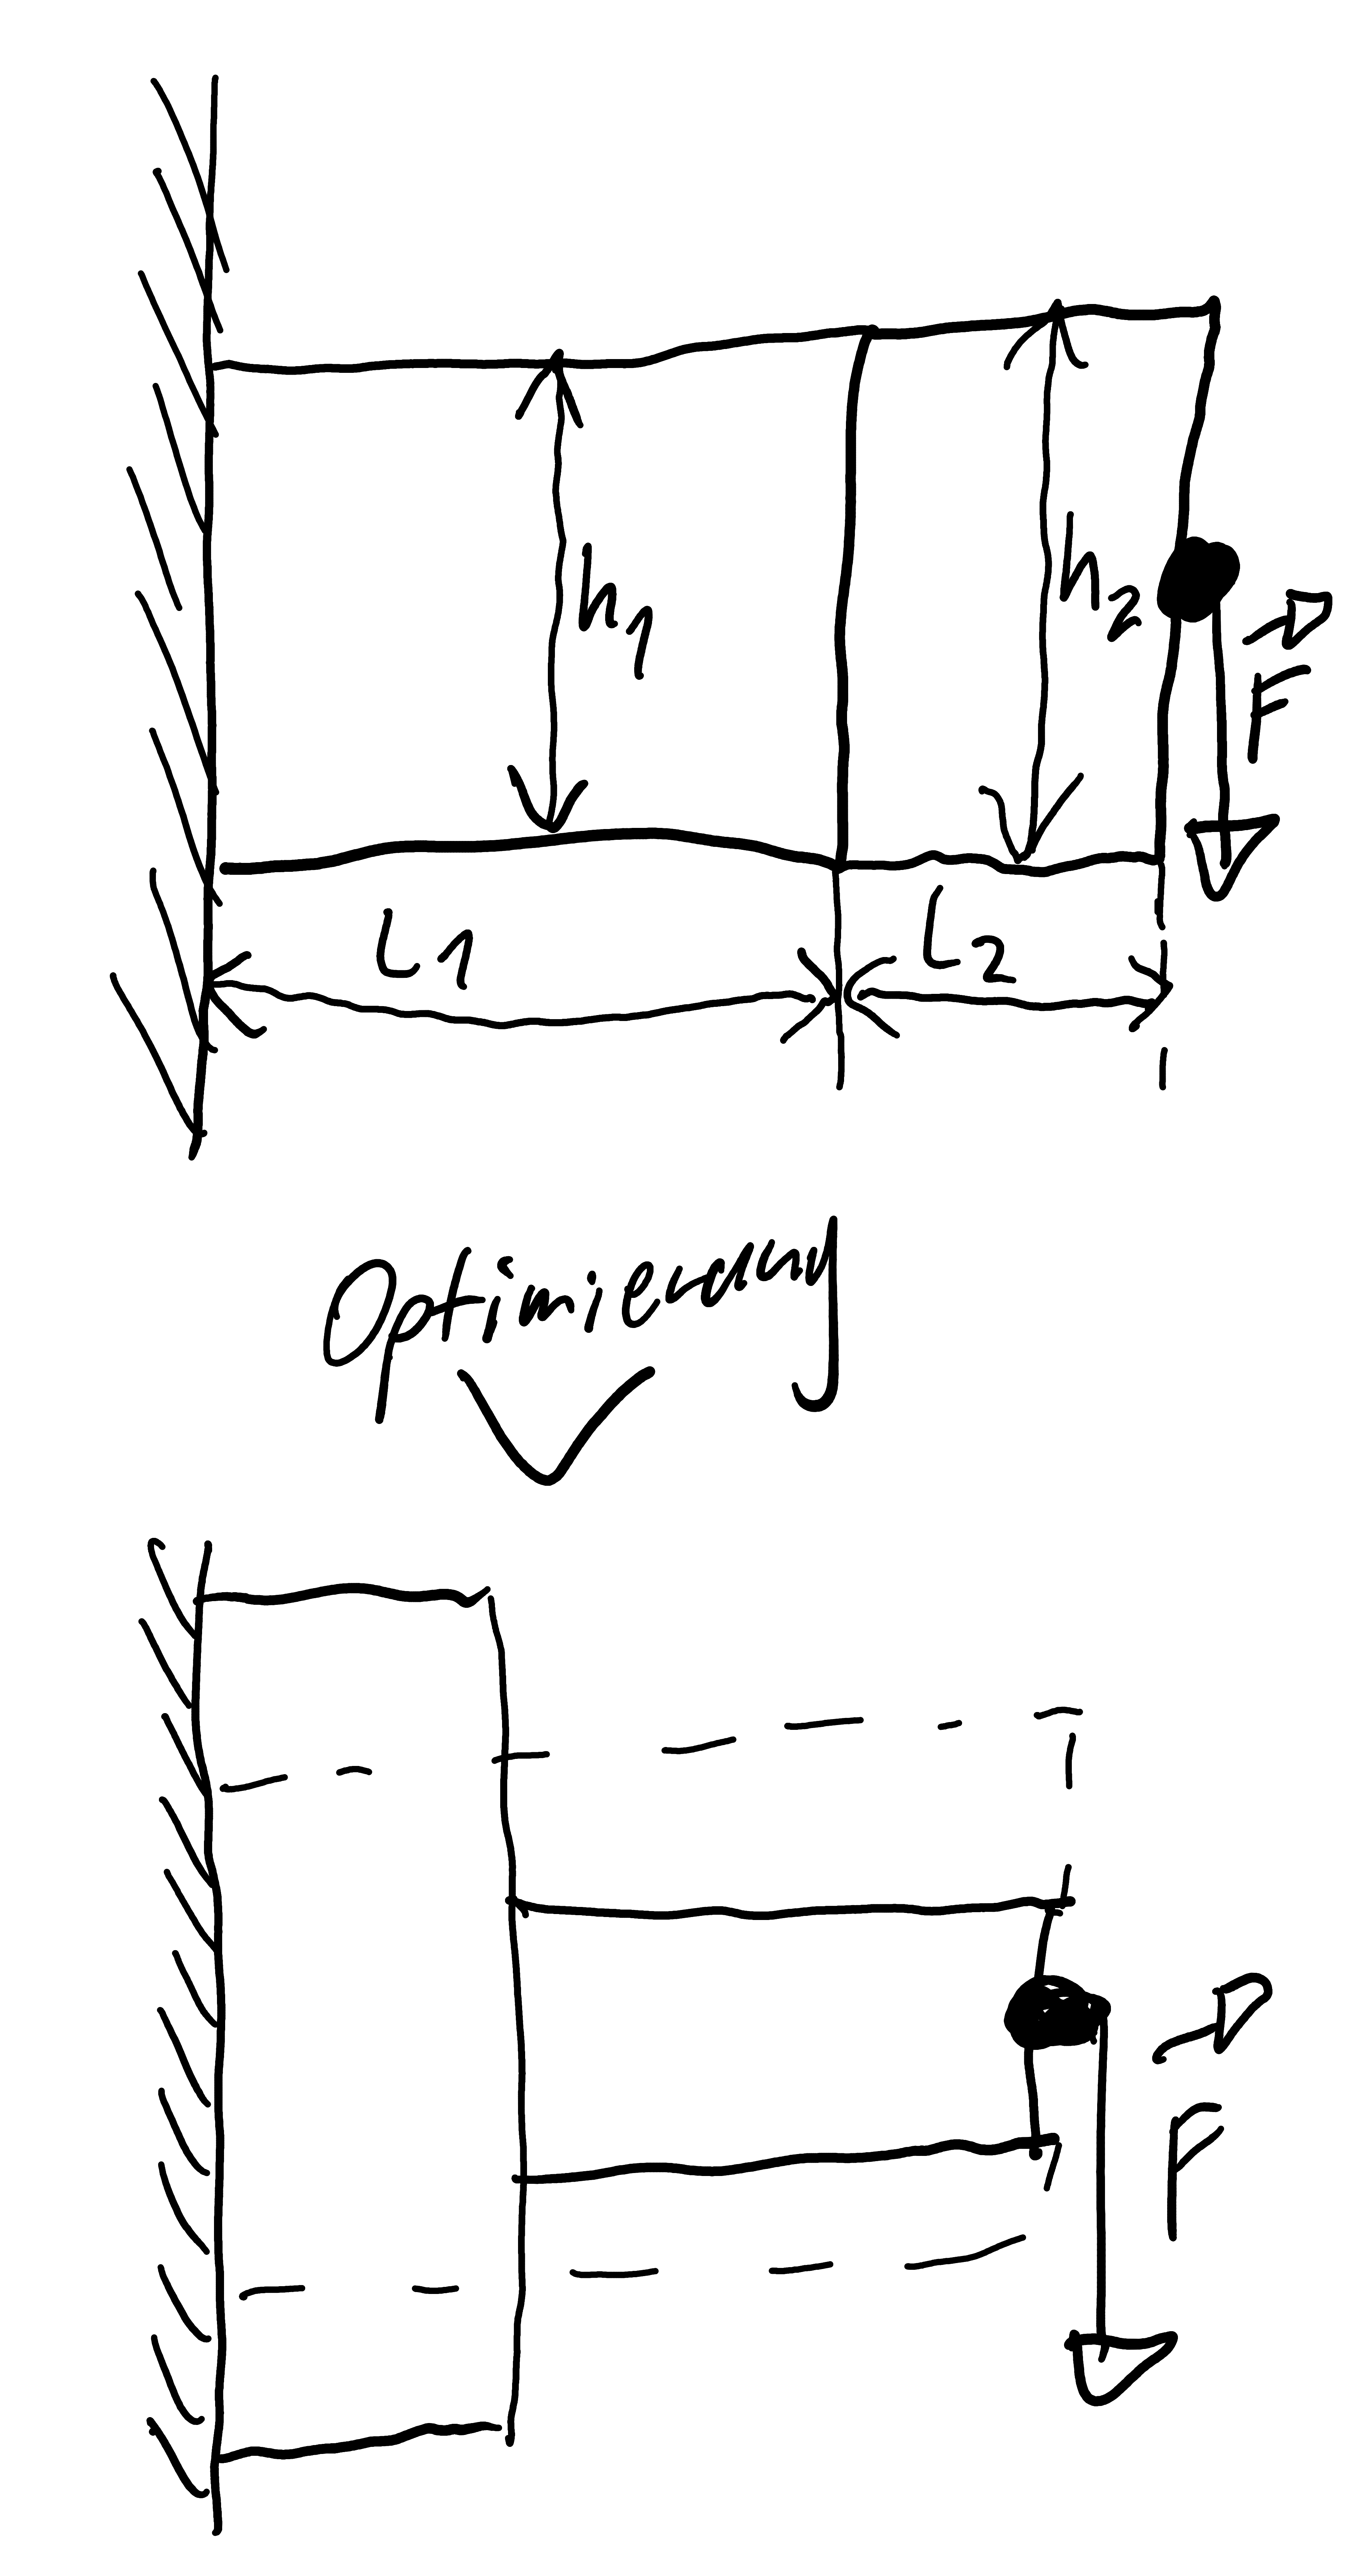
\includegraphics[width=\linewidth]{figures/Groesen-opt.png}
            \caption{Gr\"o\ss{}en Optimierung}
          \end{minipage}\hfill
          \begin{minipage}{0.2\textwidth}
            \centering
            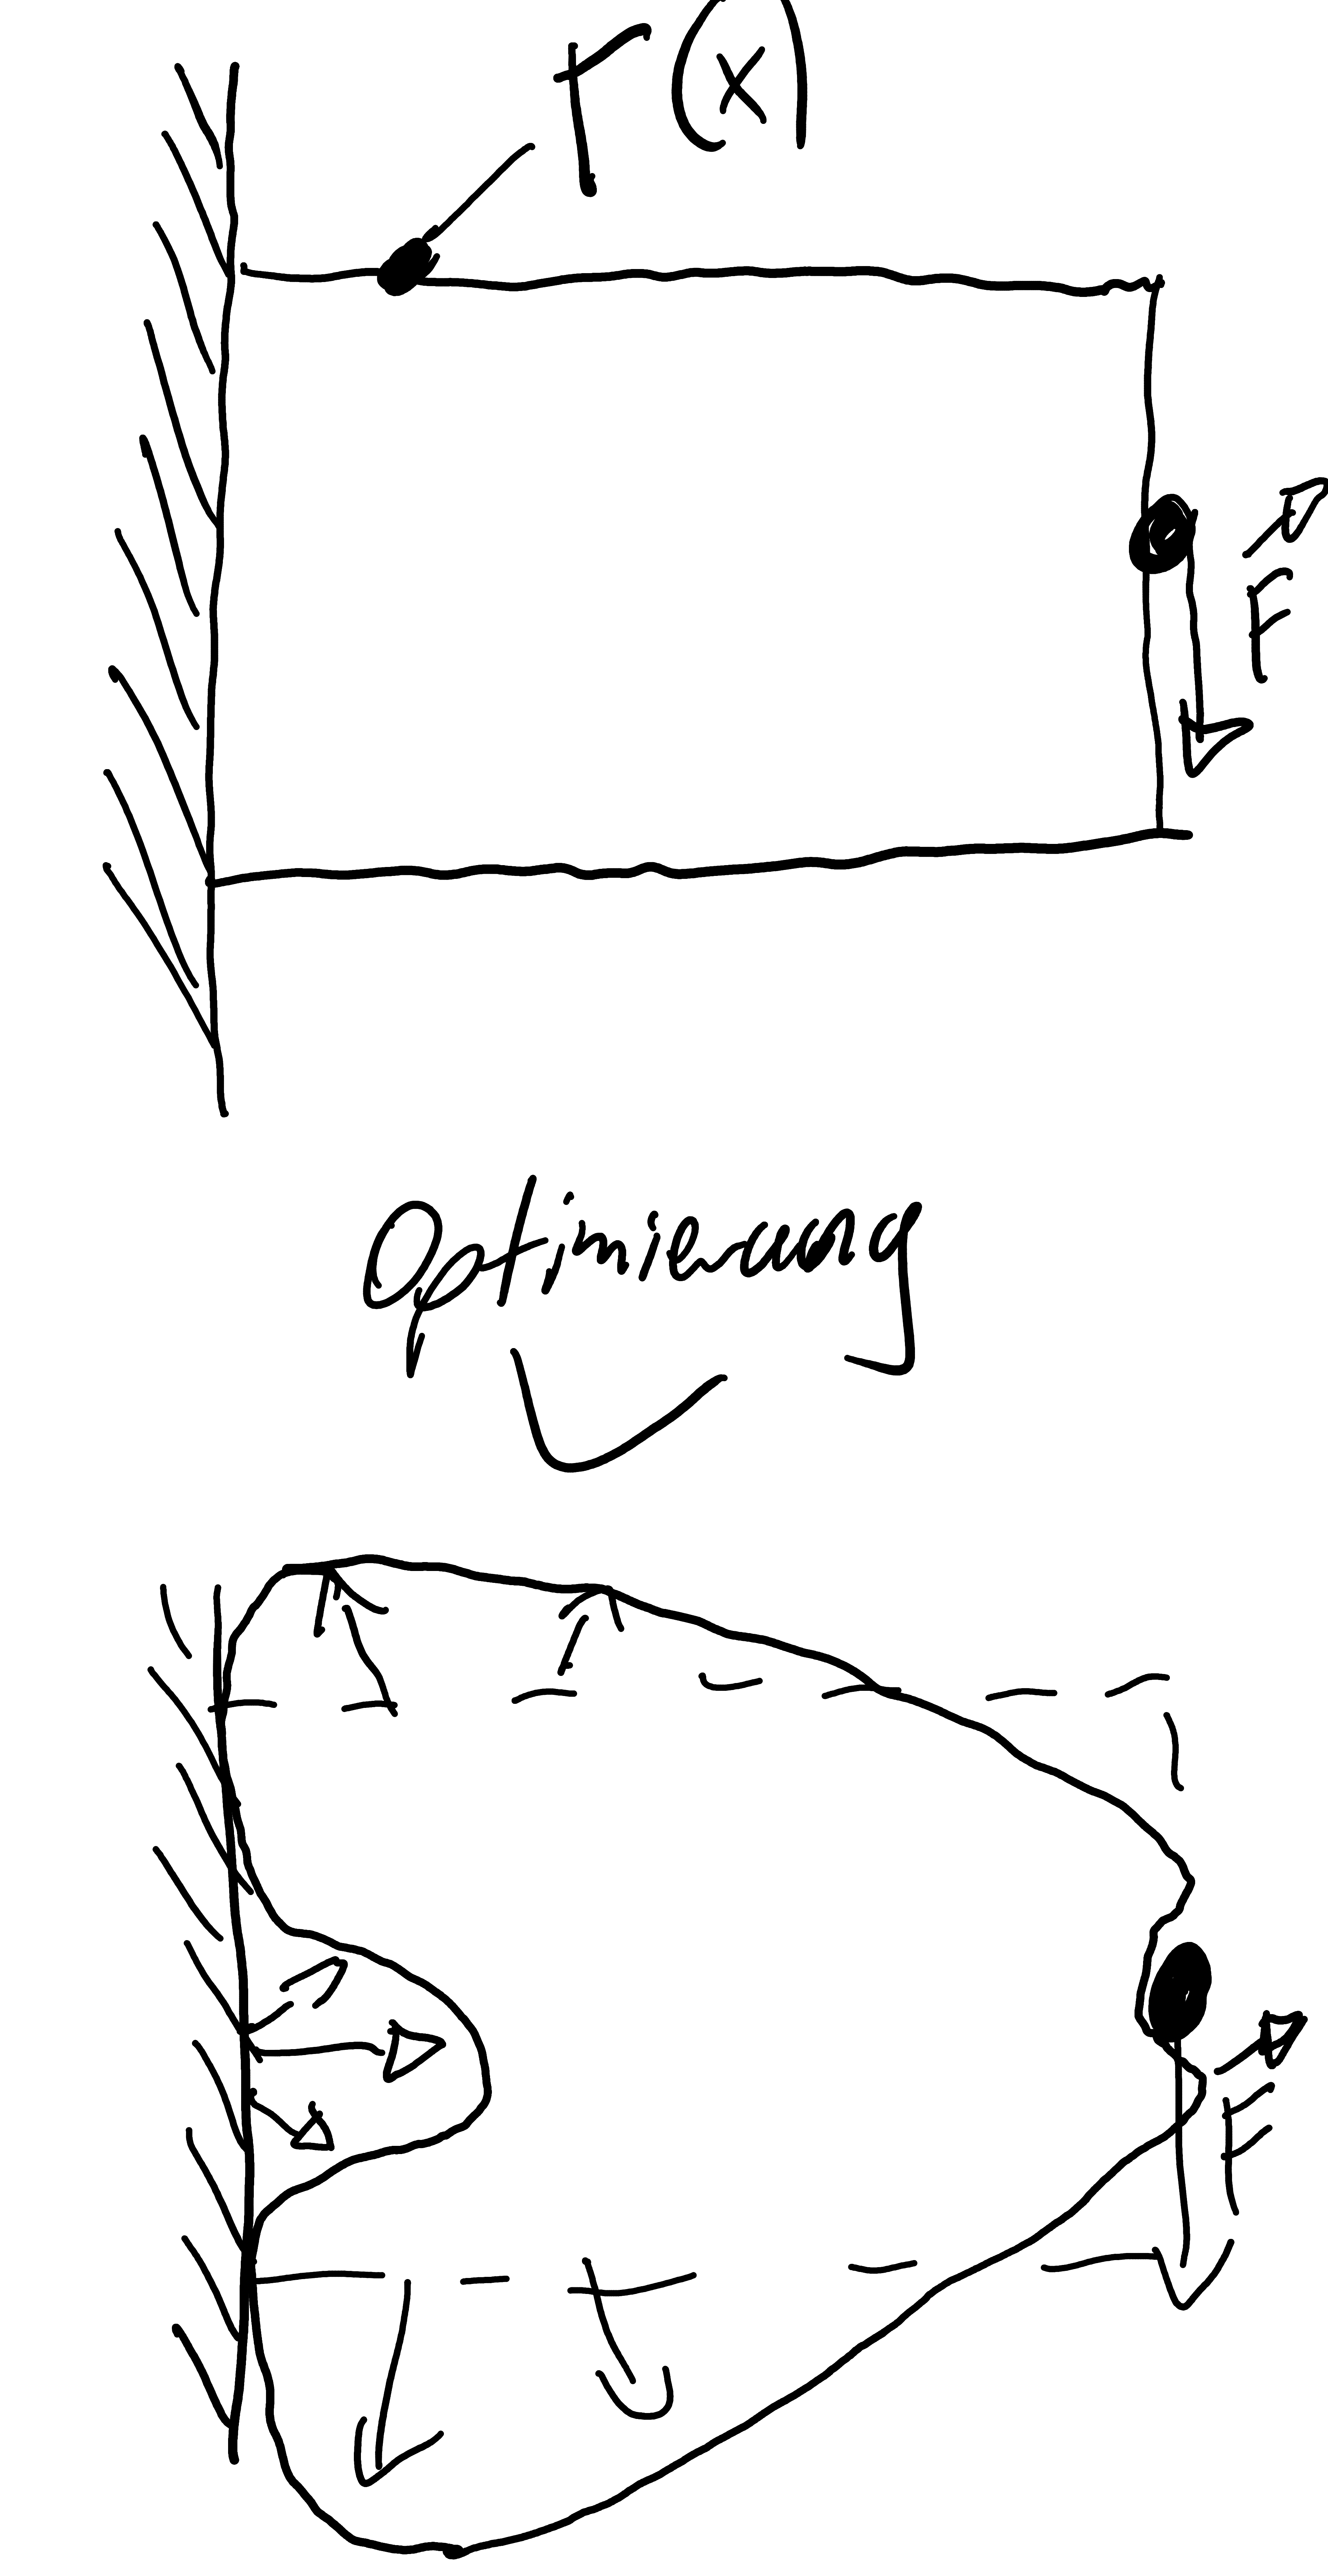
\includegraphics[width=\linewidth]{figures/Form-opt.png}
            \caption{Form Optimierung}
          \end{minipage}\hfill
          \begin{minipage}{0.2\textwidth}
            \centering
            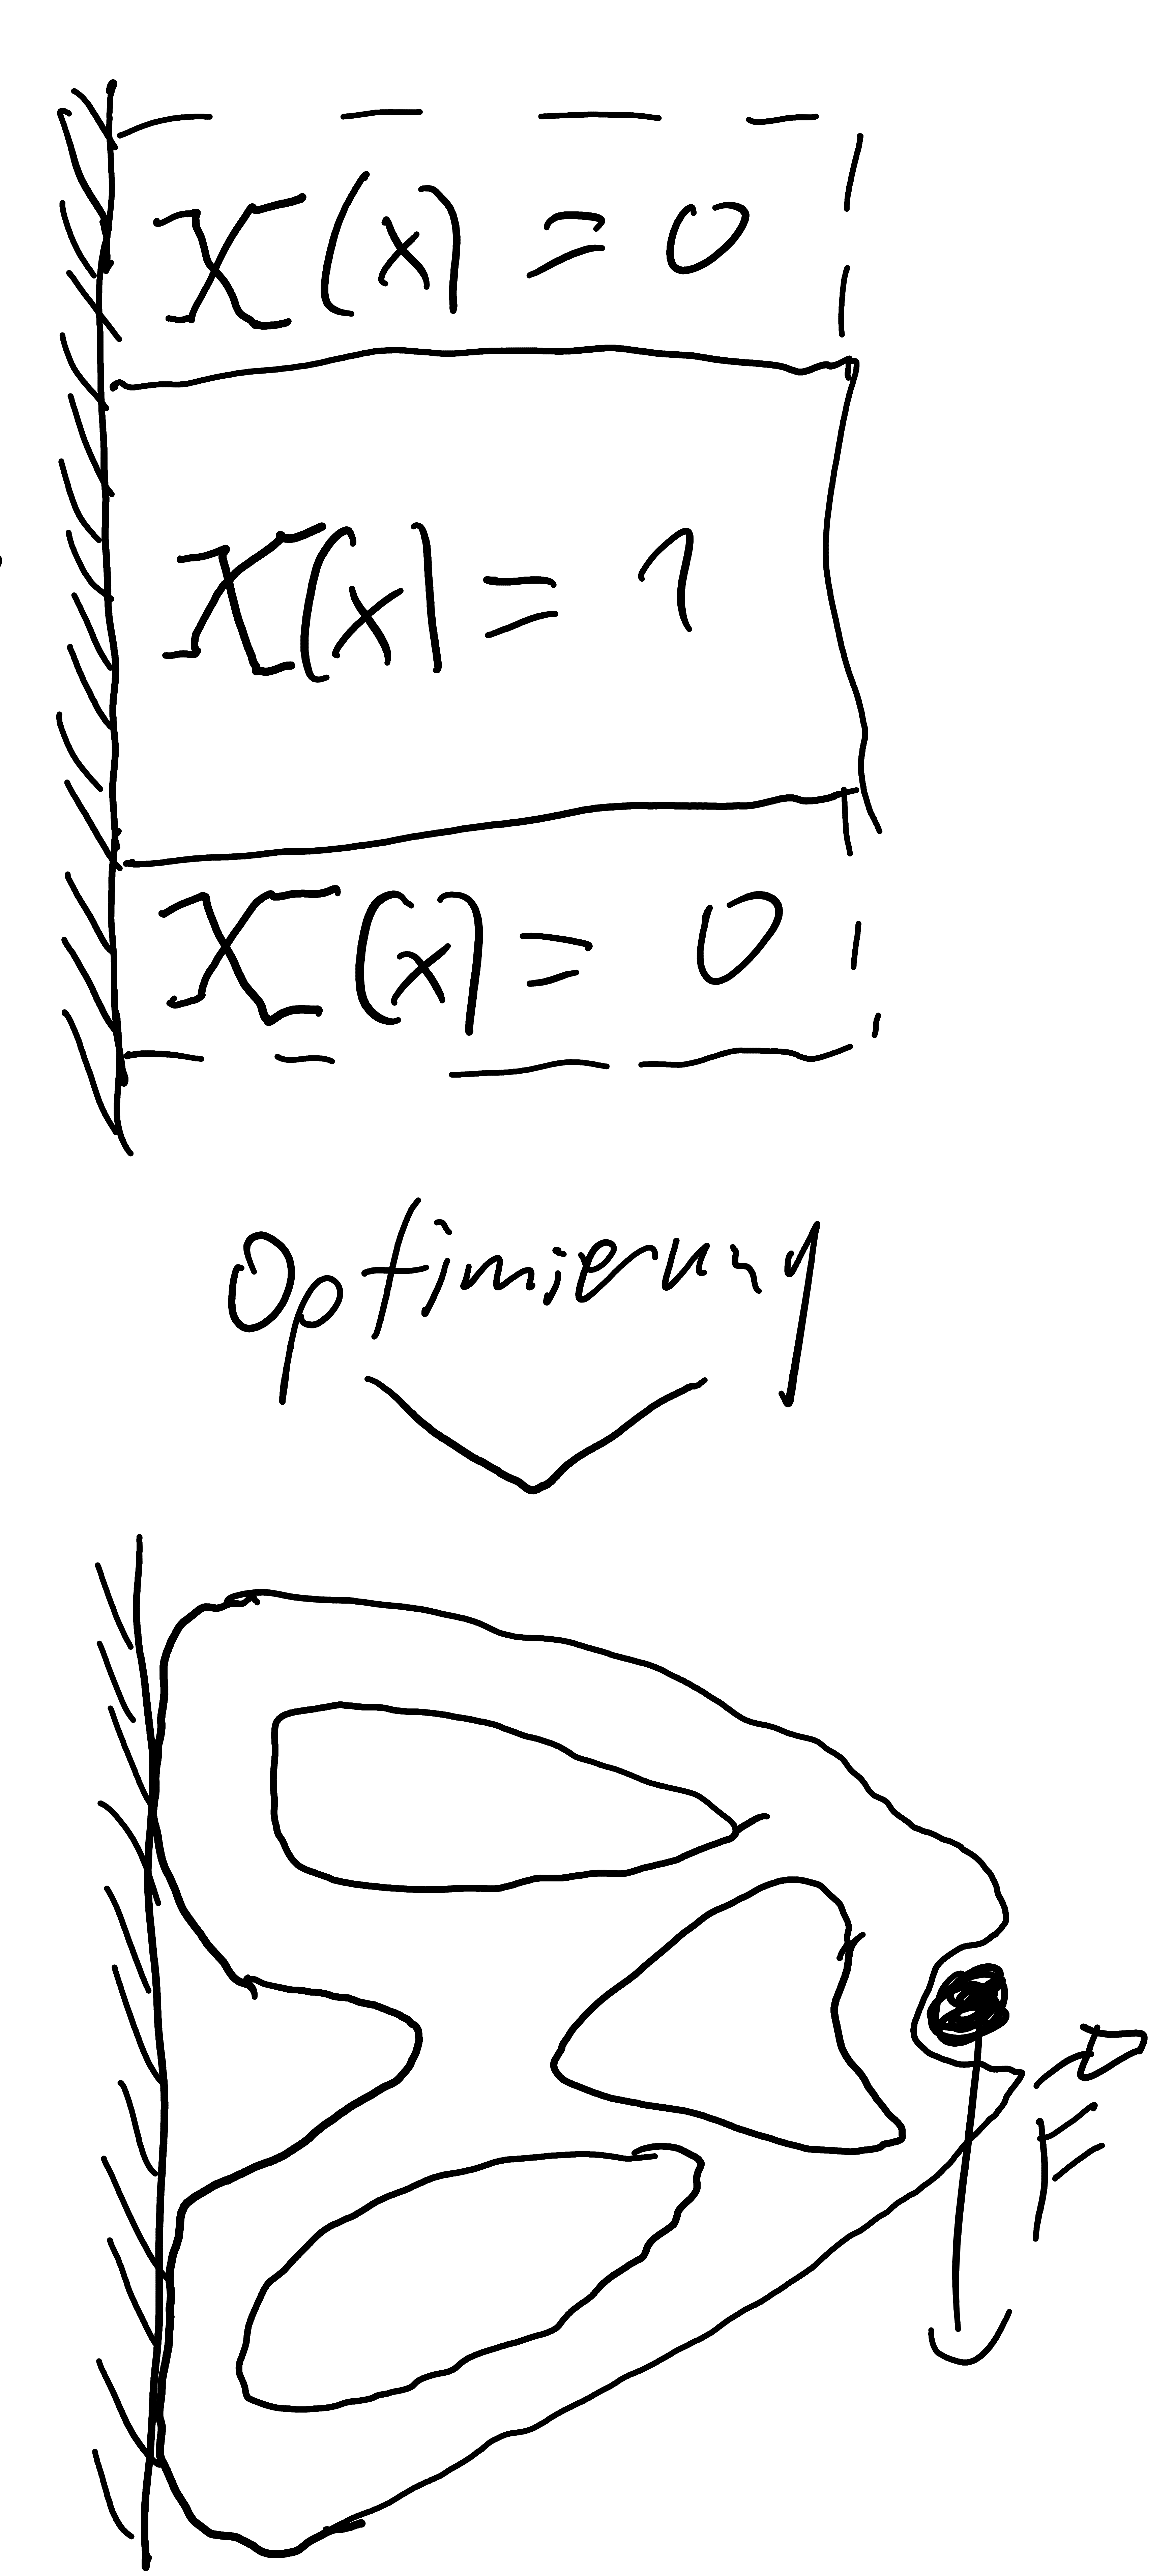
\includegraphics[width=\linewidth]{figures/Topo-opt.png}
            \caption{Topologische Optimierung}
          \end{minipage}
    \caption{Unterschied zwischen verschiedenen Optimierungen}
    \label{fig:unterschied}
\end{figure}

Mit der Abbildung wird klar wie optimiert wird, wo die Gr\"o\ss{}en
Optimierungen nur zwei Parameter je Rechteck \"andern kann, kann die
Form-Optimierung sich von der Geometrischen ``Vorgaben'' des Rechtecks L\"osen.
Die Topologische Optimierung ist dann im Stande sich von der
Homotopieäquivalenzklasse\footnote{Grob gesagt: Anzahl der L\"ocher} zu
l\"osen, dies ist dann der Schritt in dem das meiste Material gespart werden kann.

\subsection{Herleitung der \"Anderung}
Aus der erkl\"arung Topologischer Optimierungen in Sektion \ref{sec:topo-opt}
geht noch nicht hervor wie diese Homotopieäquivalenzklassen \"Anderung zustande
kommt, dies wird in dieser Sektion langsam erkl\"art.

Bei topologischen Optimierungen sind ein paar Formeln und Faktoren
entscheident, angefangen mit der Kostenfunktion
\begin{equation}
    c=\frac{1}{2}U^{T}K\cdot \vec{U}
\end{equation}
Hier repr\"asentiert $c$ das Konstenma\ss{}, $\vec{U}$ Verschiebung und
Deformation in einem System, $K$ eine Steifigkeits-, bzw. Elastizit\"atsmatrix
und $U^T$ die transponierte Form des Vektors. 

Dem kann man dann entnehmen das die Multiplikation $U^TKU$ eine quadratische
Form die in der Elastizit\"atstheorie und Finite-Element-Analyse verwendet wird.

Die n\"achste essentielle Formel ist f\"urdie Elastische Energie:
\begin{equation}
   c=\frac{1}{2}fu=\frac{1}{2}ku^2 
\end{equation}
hier repr\"asentiert $c$ die elastische Energie, $f$ die auf das System
ausge\"ubte Kraft, $u$ die Deformation im System und $k$ die Federkonstante des
Systems.

Zuletzt ben\"otigt man noch die Statische Gleichung:
\begin{equation}
    k\vec{u}=f
\end{equation}
Hier ist $k$ die Steifigkeitsmatrix bzw. Federkonstante~\footnote{Abh\"angig
von der Anzahl der zu ber\"ucksichtigen Dimensionen.}, $\vec{u}$ die Verformung
im System und $f$ die auf das System ausge\"ubte Kraft.

Diese sind dann Final von einigen Bedingungen abh\"angig:
\begin{itemize}
    \item $ku = F$: Diese Formulierung repräsentiert die statische
        Gleichgewichtsgleichung, die besagt, dass die resultierende Verformung
        $u$ im System gleich der externen angewandten Kraft $F$ ist. 

    \item $\rho_i \in \{1 \text{ (vorhanden)}, 0 \text{ (leer)}\}, \quad
        \forall i$: Dies gibt an, dass $\rho_i$ entweder den Wert 1 (vorhanden)
        oder 0 (leer) haben kann. Dabei repräsentiert $i$ die einzelnen
        Elemente des Systems.

    \item $g = \sum_i \rho_i - V_0 \leq 0$: Dies ist die letzte Nebenbedingung,
        die besagt, dass die Summe der $\rho_i$ Werte minus $V_0$ kleiner oder
        gleich null sein muss, wobei $V_0$ eine bestimmte Schwelle für das
        Erscheinen der Elemente im System darstellt.
\end{itemize}


\subsection{Simulation}
Die letzte einf\"uhrende Sektion wird sich mit einer Simulations Software
\parencite{aage2014} der Deanmarks Tekniske Universitet (Techinische Universit\"at D\"anemark)
besch\"aftigen, diese ist zwei-Dimensional und gut um Zusammenh\"ange intuitiv zu zeigen.

Ich werde einige Beispiele zeigen und empfehle, dass wenn Interesse besteht man es selbst versucht.

\begin{figure}[H]
    \centering
    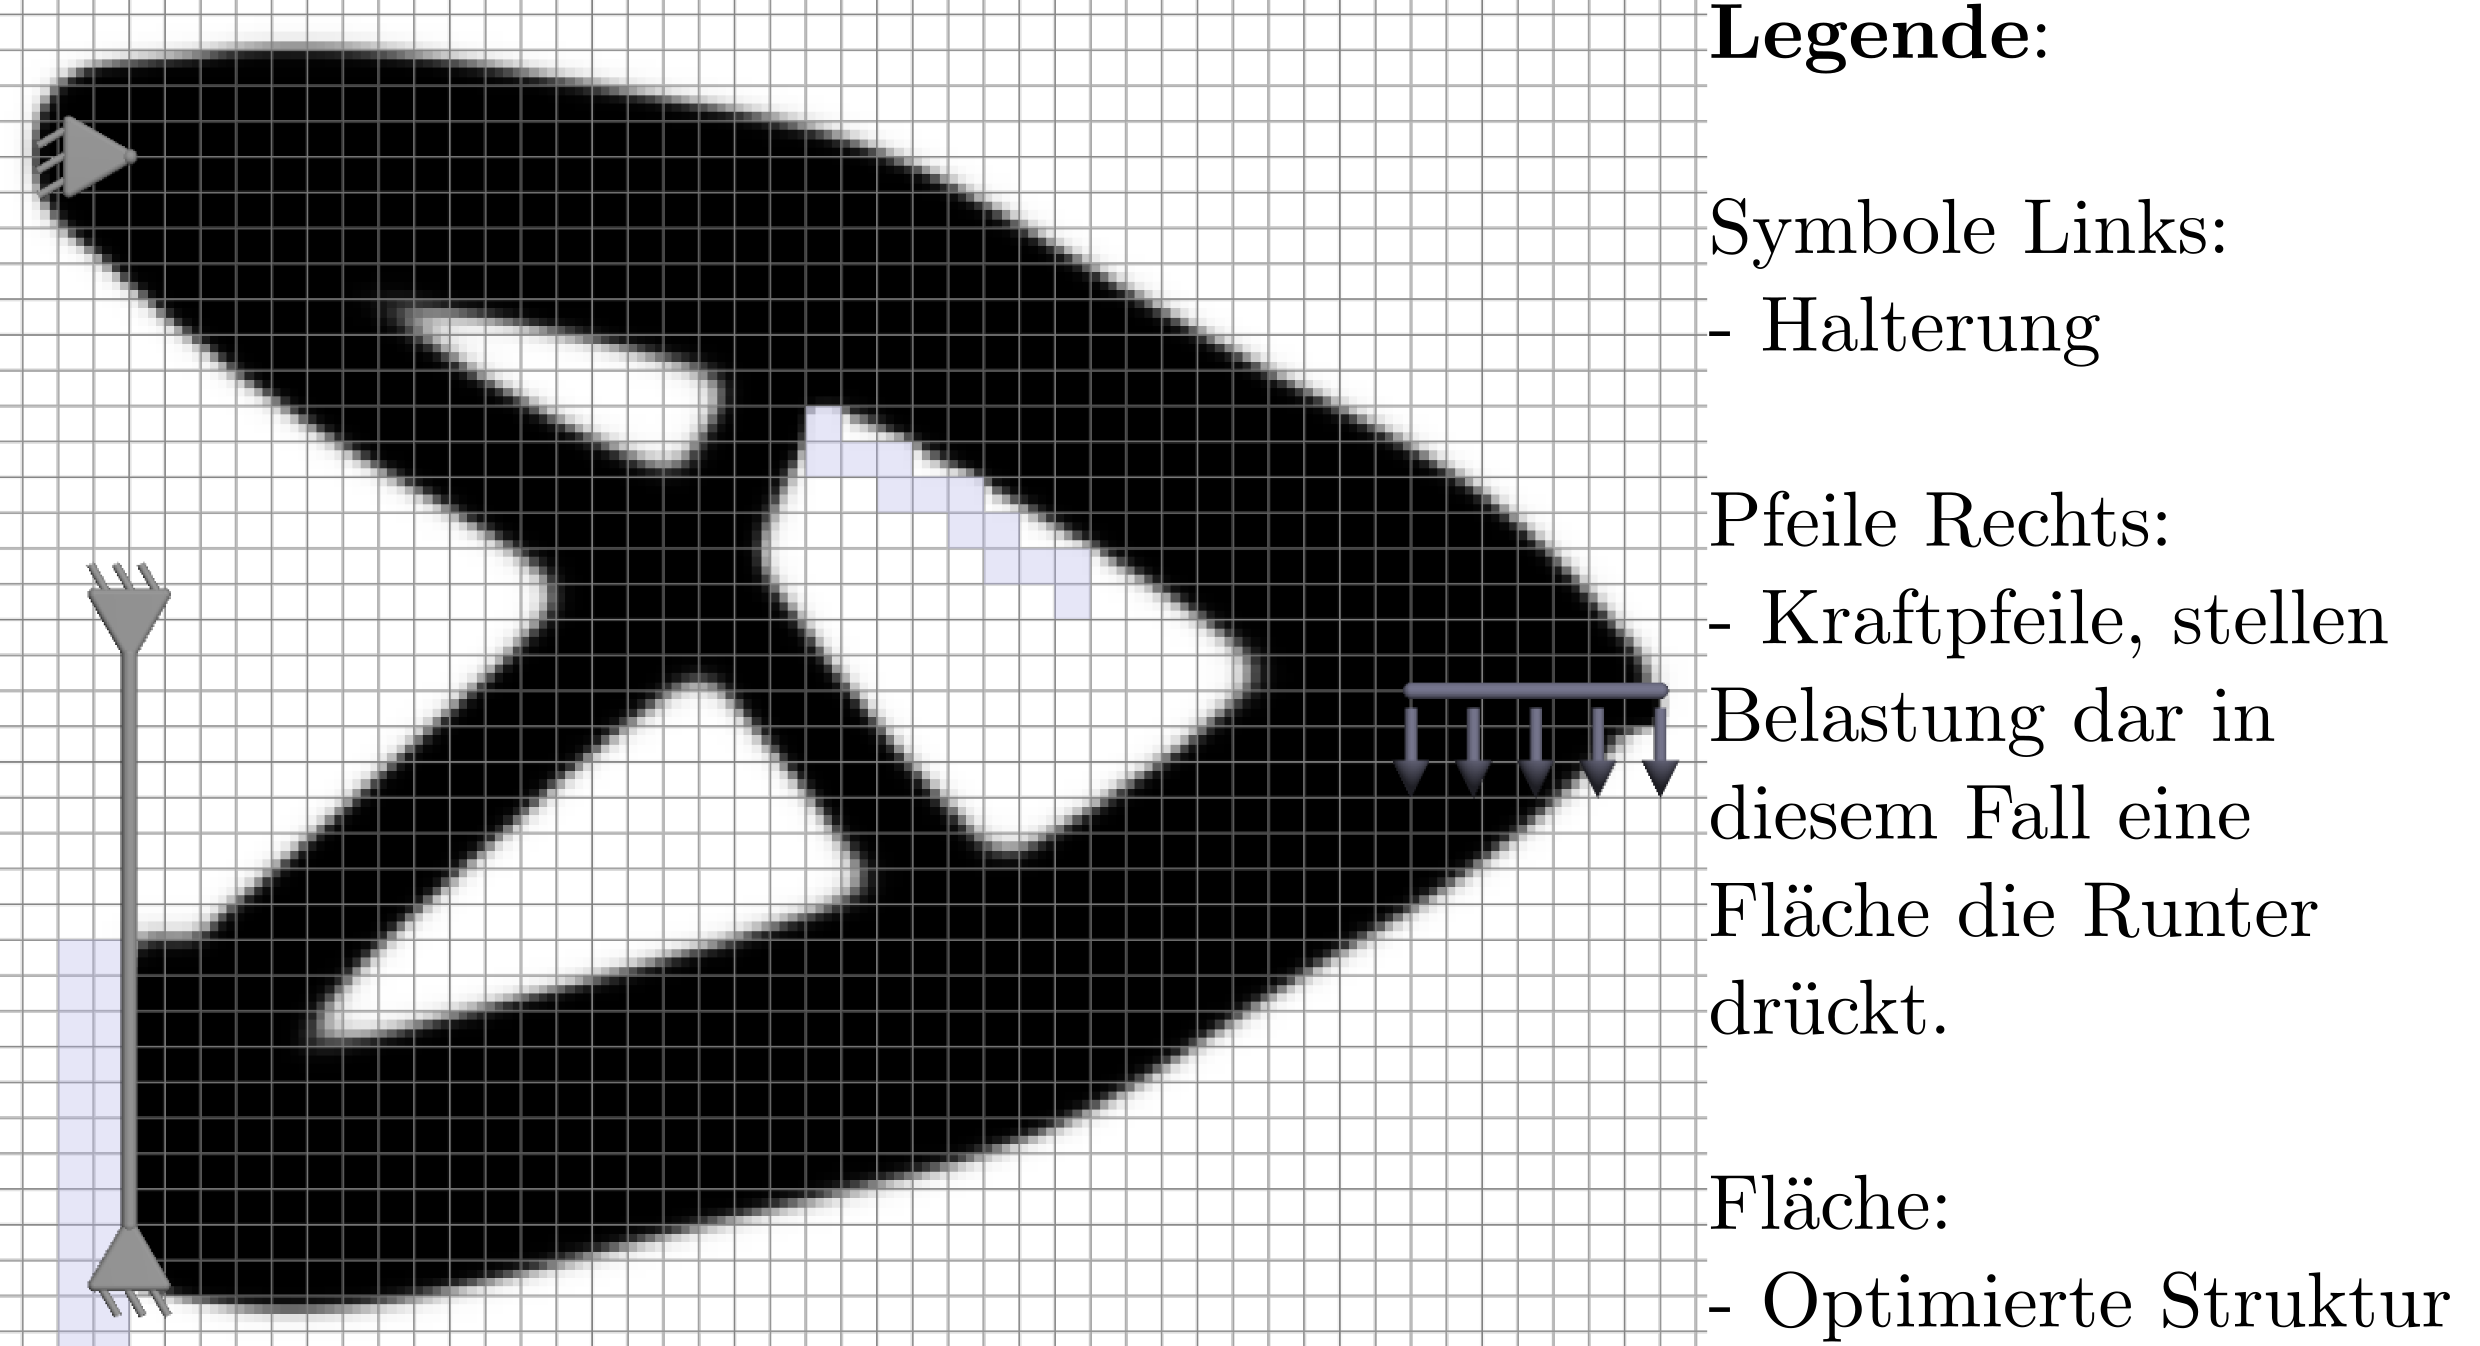
\includegraphics[width=1\textwidth]{figures/legende.png}
    \caption{Legende zur Simulation}
    \label{fig:legende}
\end{figure}

Um es nochmal zu erw\"ahnen, die schwarzen Strukturen sind komplett nach den Angezeigten 
Parametern generiert.

\begin{figure}[H]
    \begin{minipage}{0.25\textwidth}
        \centering
        \includegraphics[width=\linewidth]{figures/brücke.png}
        \caption{Br\"ucke}
        \label{fig:bruecke}
    \end{minipage}\hfill
    \begin{minipage}{0.25\textwidth}
        \centering
        \includegraphics[width=\linewidth]{figures/Fläche.png}
        \caption{Tragfl\"ache}
    \end{minipage}\hfill
    \begin{minipage}{0.25\textwidth}
        \centering
        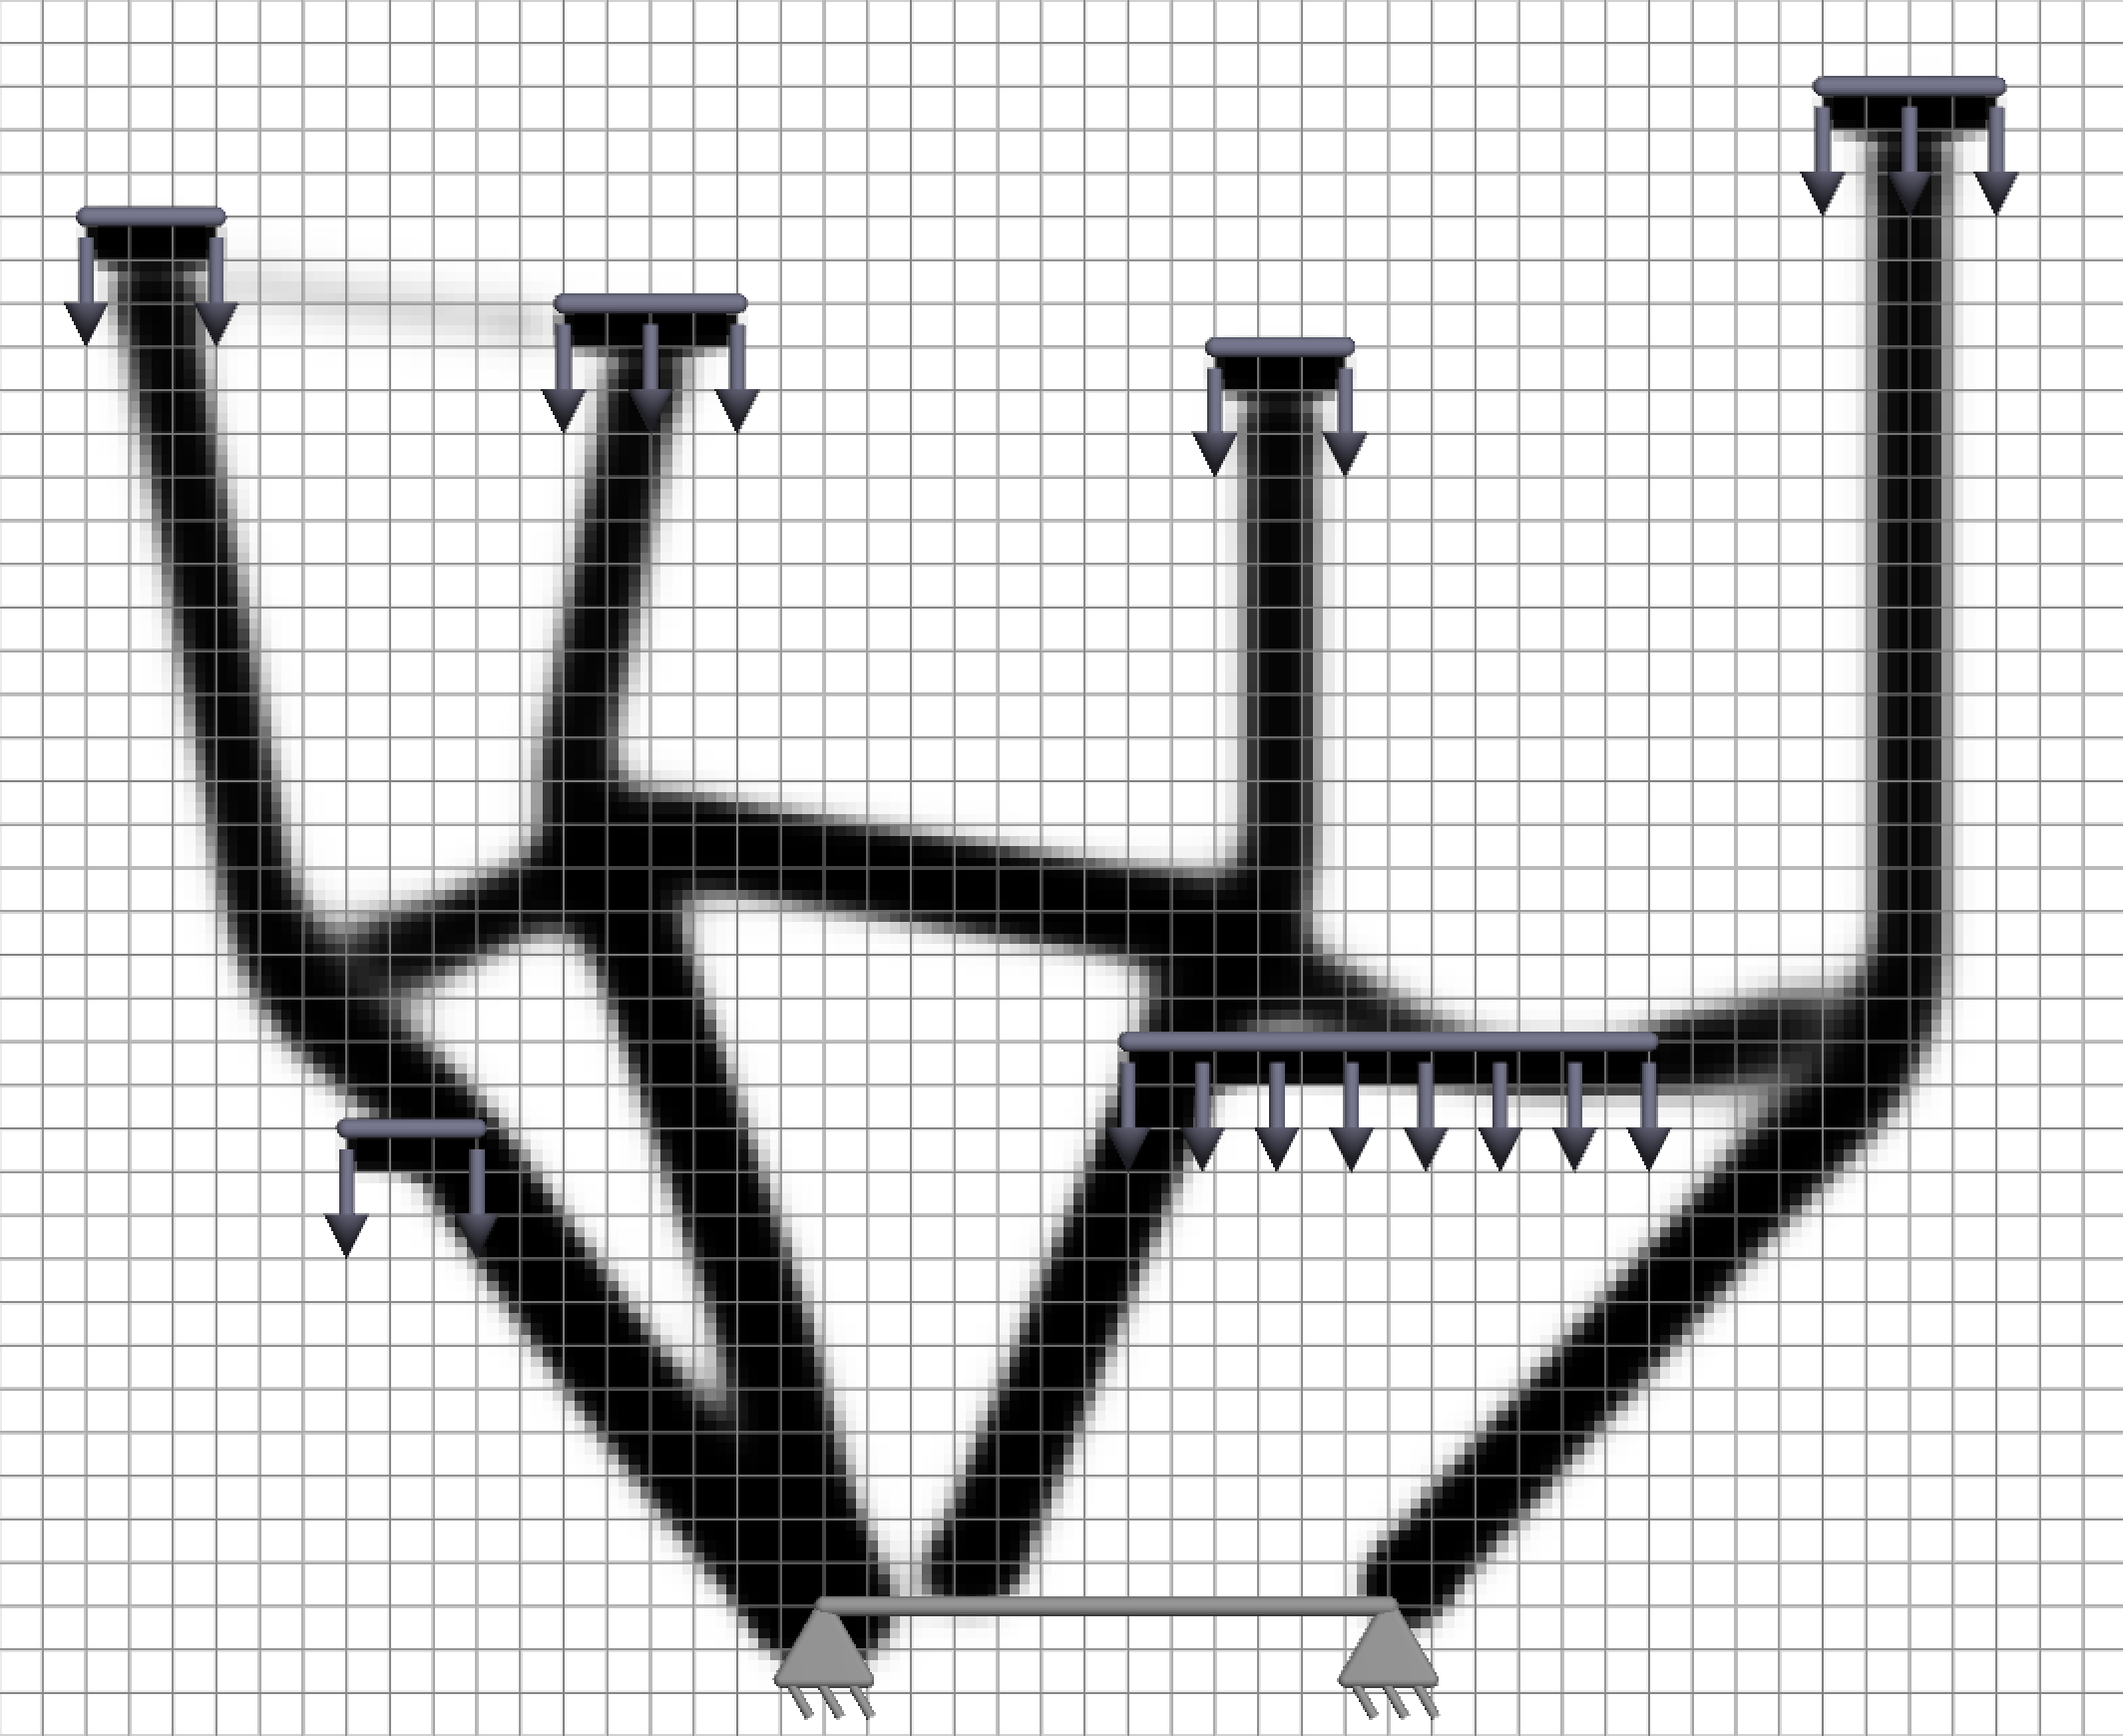
\includegraphics[width=\linewidth]{figures/baum.png}
        \caption{Baum}
    \end{minipage}
\end{figure}

\begin{figure}[H]
    \begin{minipage}{0.25\textwidth}
        \centering
        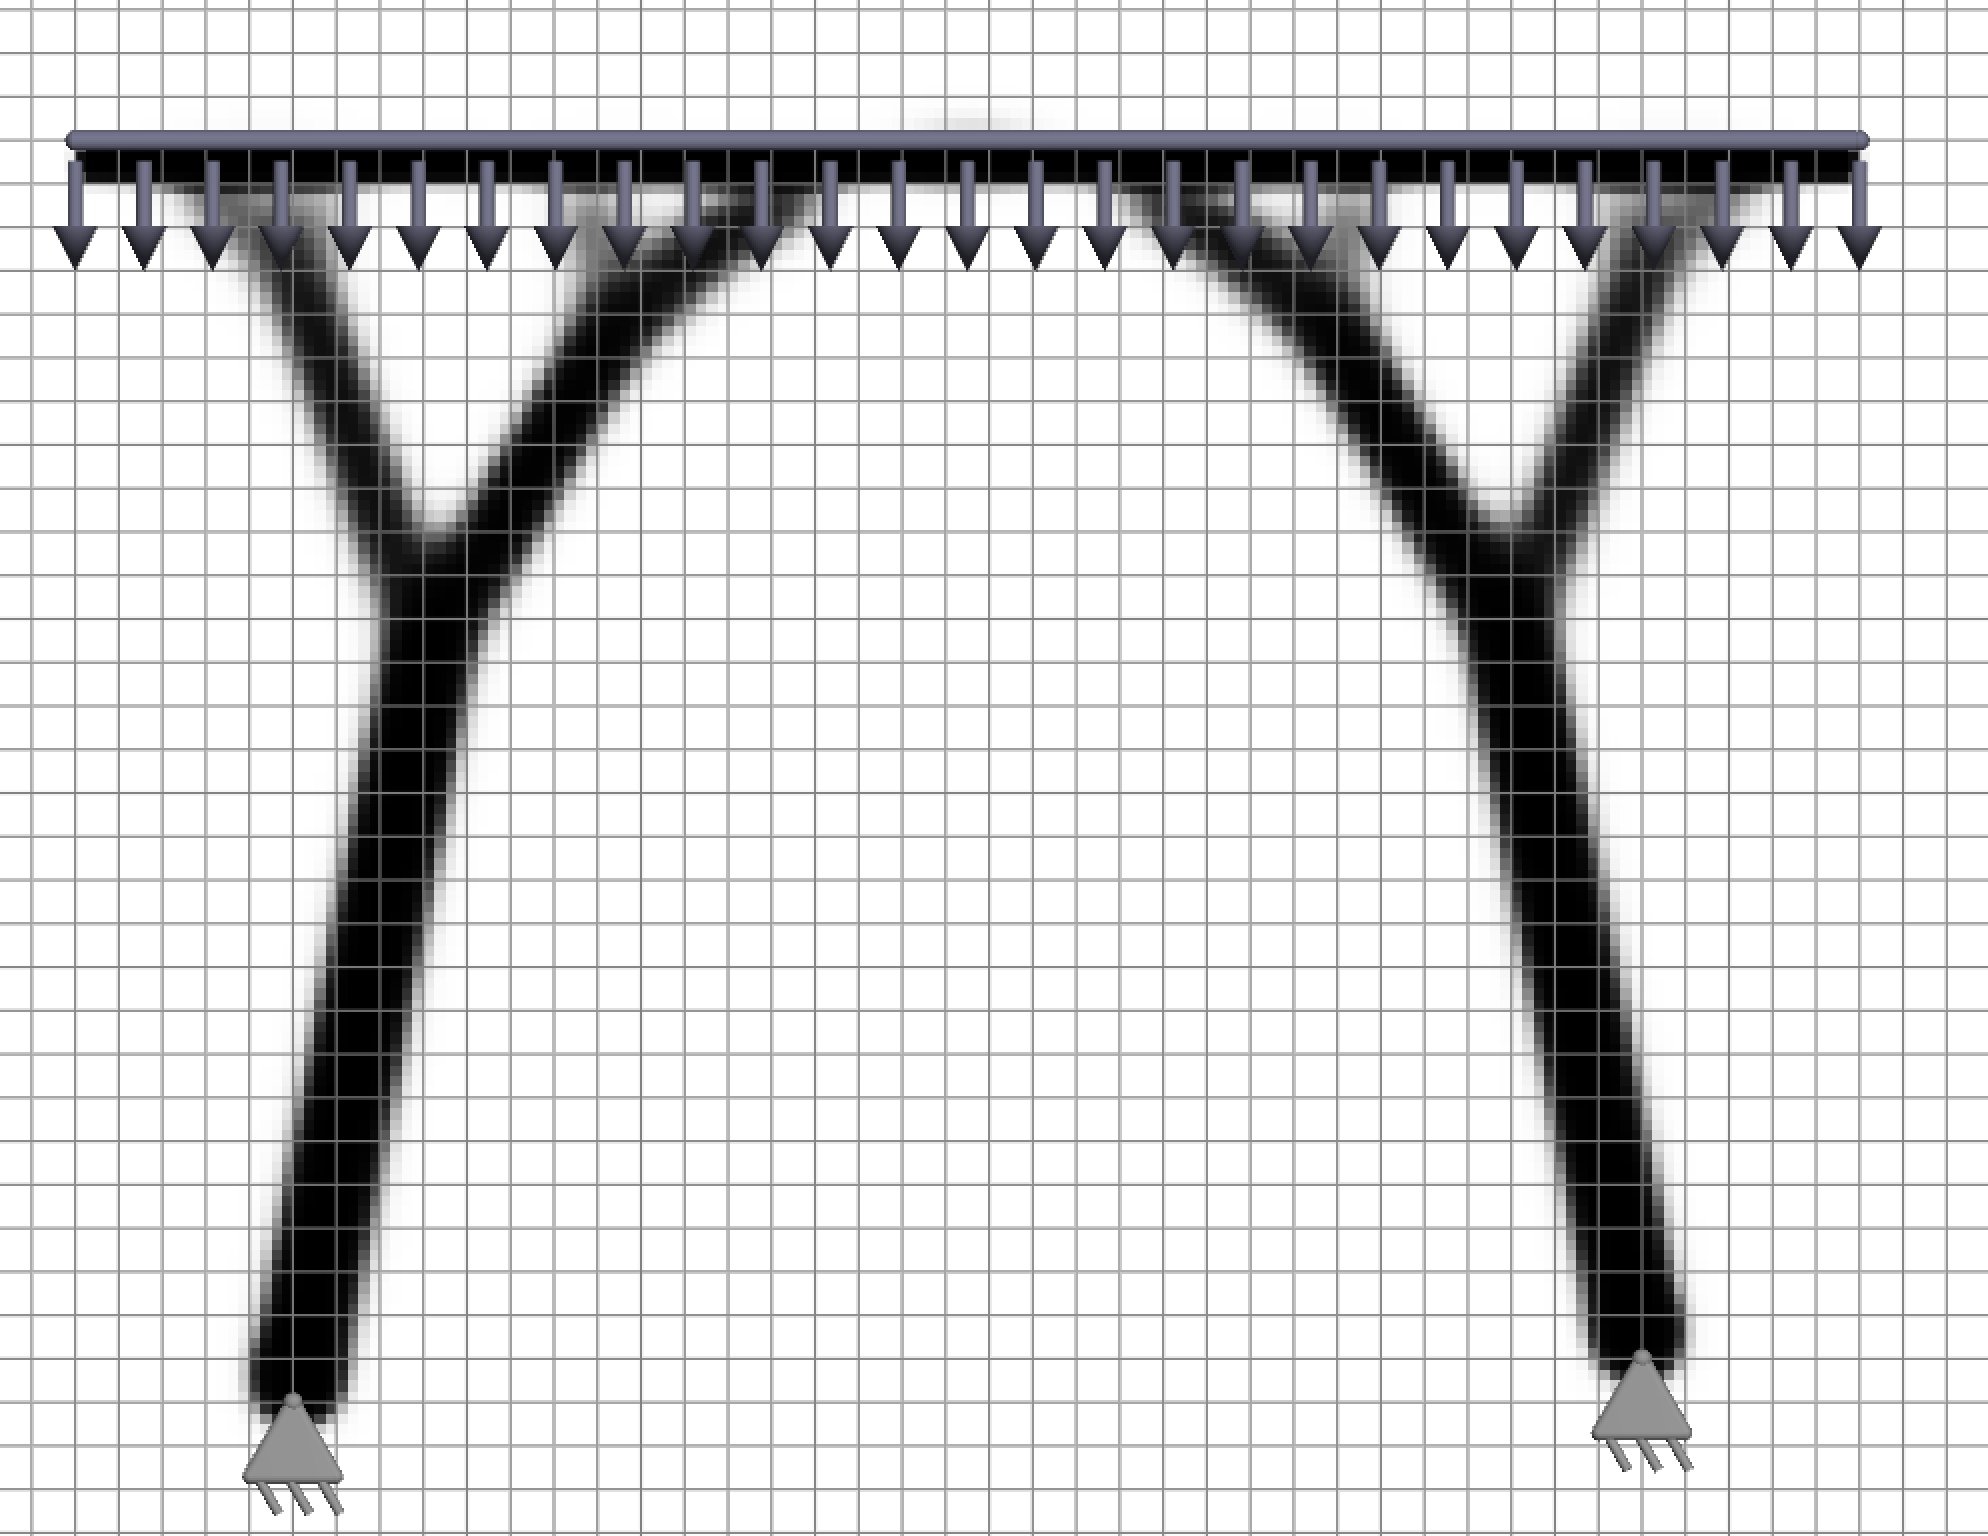
\includegraphics[width=\linewidth]{figures/tisch.png}
        \caption{Tisch}
    \end{minipage}\hfill
    \begin{minipage}{0.25\textwidth}
        \centering
        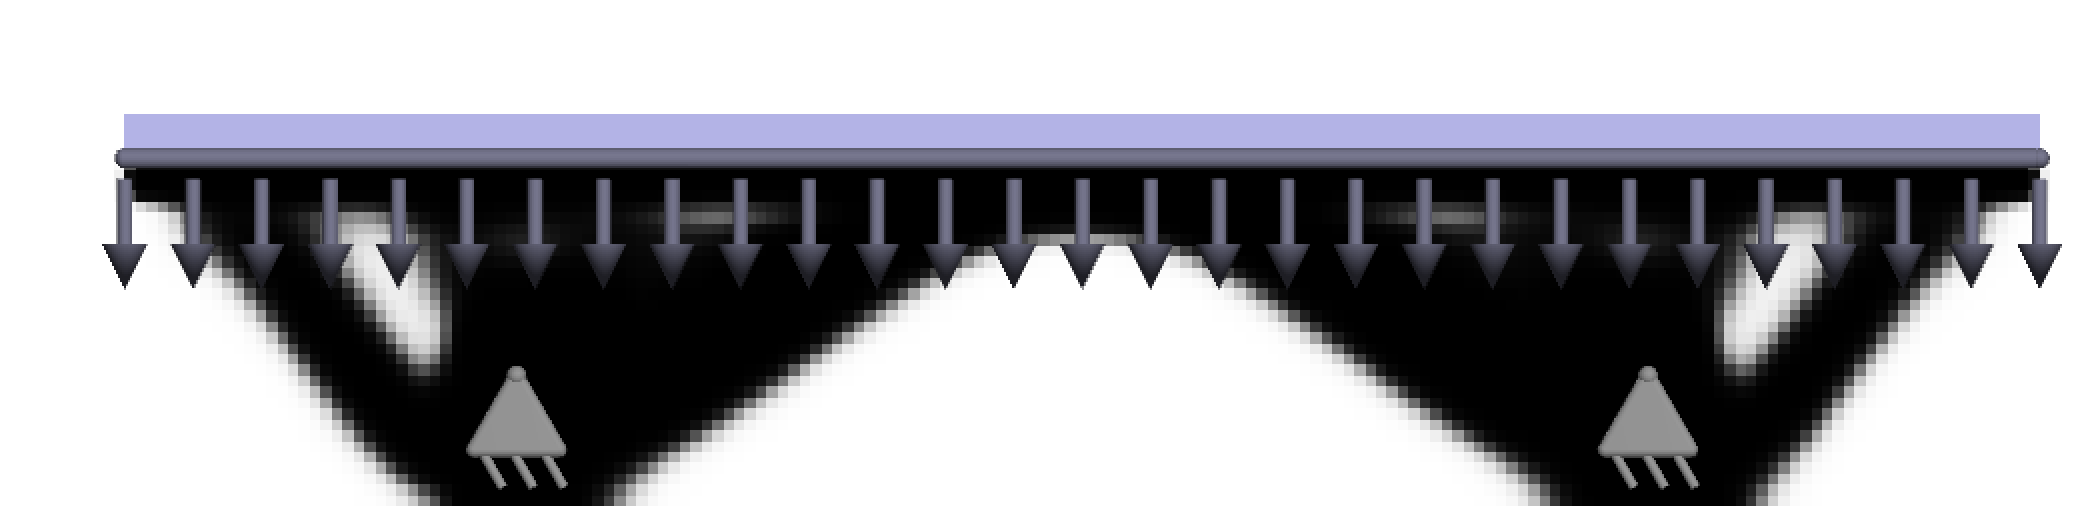
\includegraphics[width=\linewidth]{figures/Palette.png}
        \caption{Palette}
    \end{minipage}\hfill
    \begin{minipage}{0.25\textwidth}
        \centering
        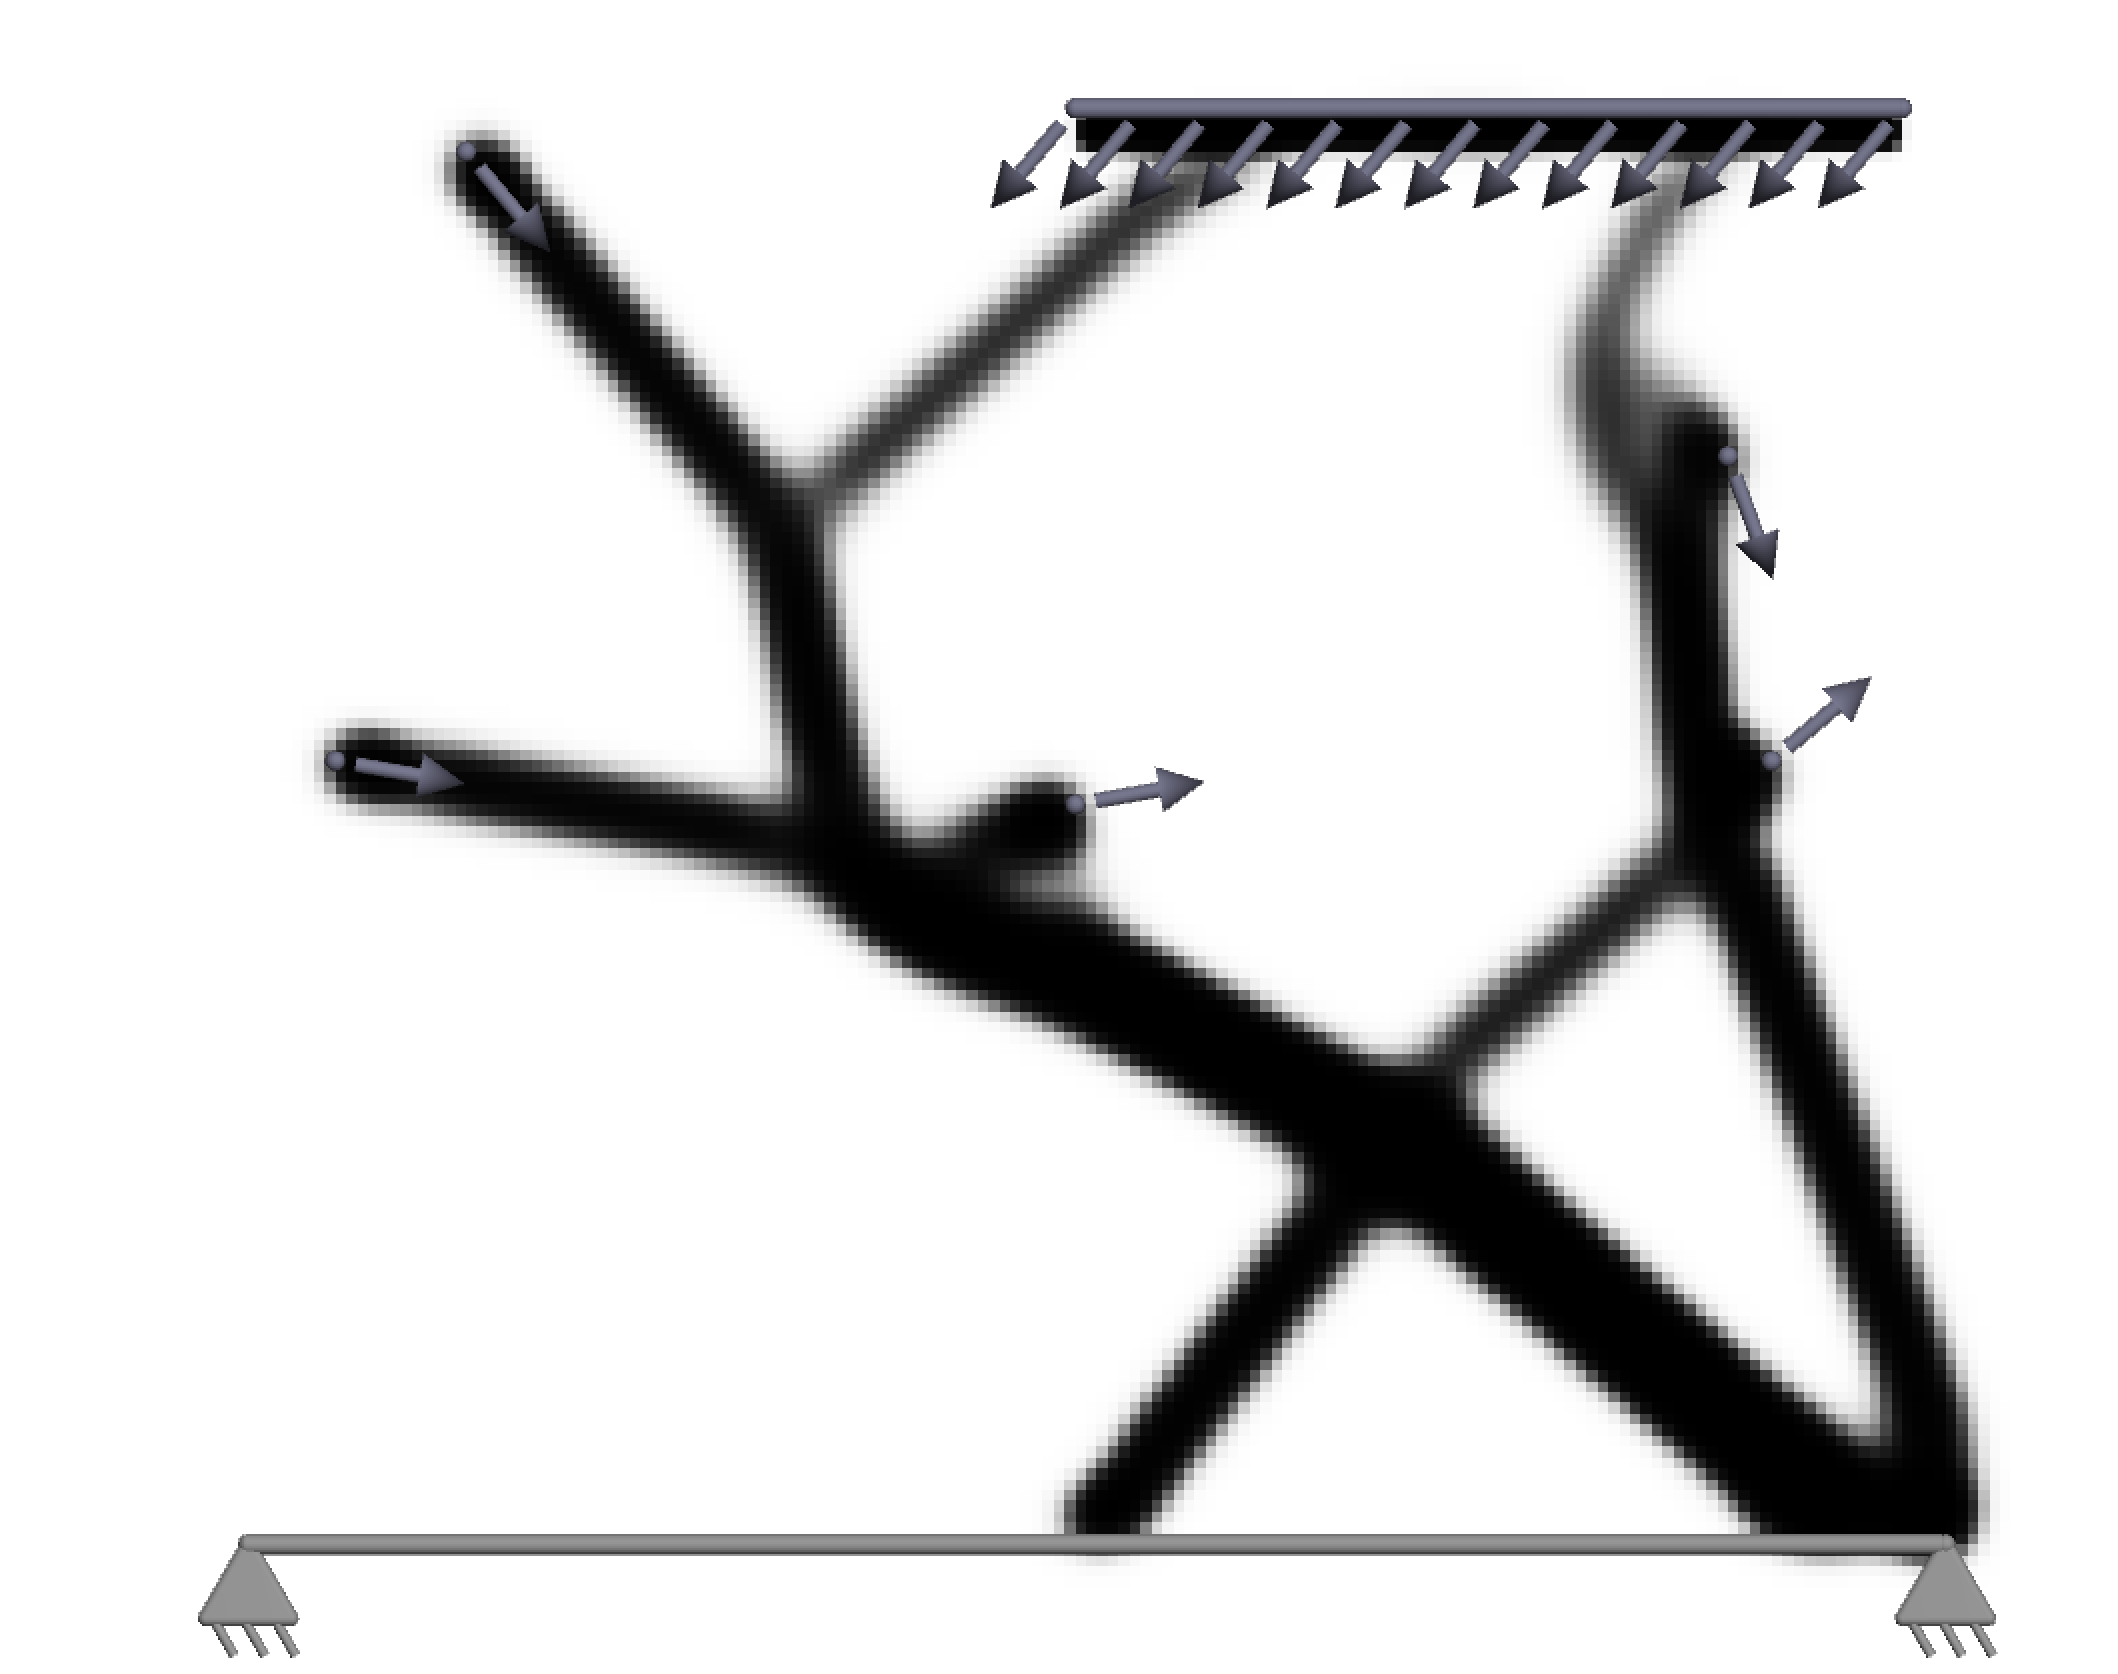
\includegraphics[width=\linewidth]{figures/abstrakt.png}
        \caption{Abstrakteres Gebilde}
        \label{fig:abstrakt}
    \end{minipage}
\end{figure}

Die Abbildungen \ref{fig:bruecke} bis \ref{fig:abstrakt} sind benannt nach
Dingen die sie evtl. zeigen k\"onnten, was ich am spannensten fand war die
Br\"ucke welche tats\"achlich wie eine normale Br\"ucke aussieht da Statiker 
und Ingeneure sehr viel Zeit f\"ur die Verbesserung der Struktur verwendeten.

\begin{figure}[H]
    \begin{minipage}{0.4\textwidth}
        \centering
        \includegraphics[width=\linewidth]{figures/brücke.png}
        \caption{Simulierte Br\"ucke}
    \end{minipage}\hfill
    \begin{minipage}{0.4\textwidth}
        \centering
        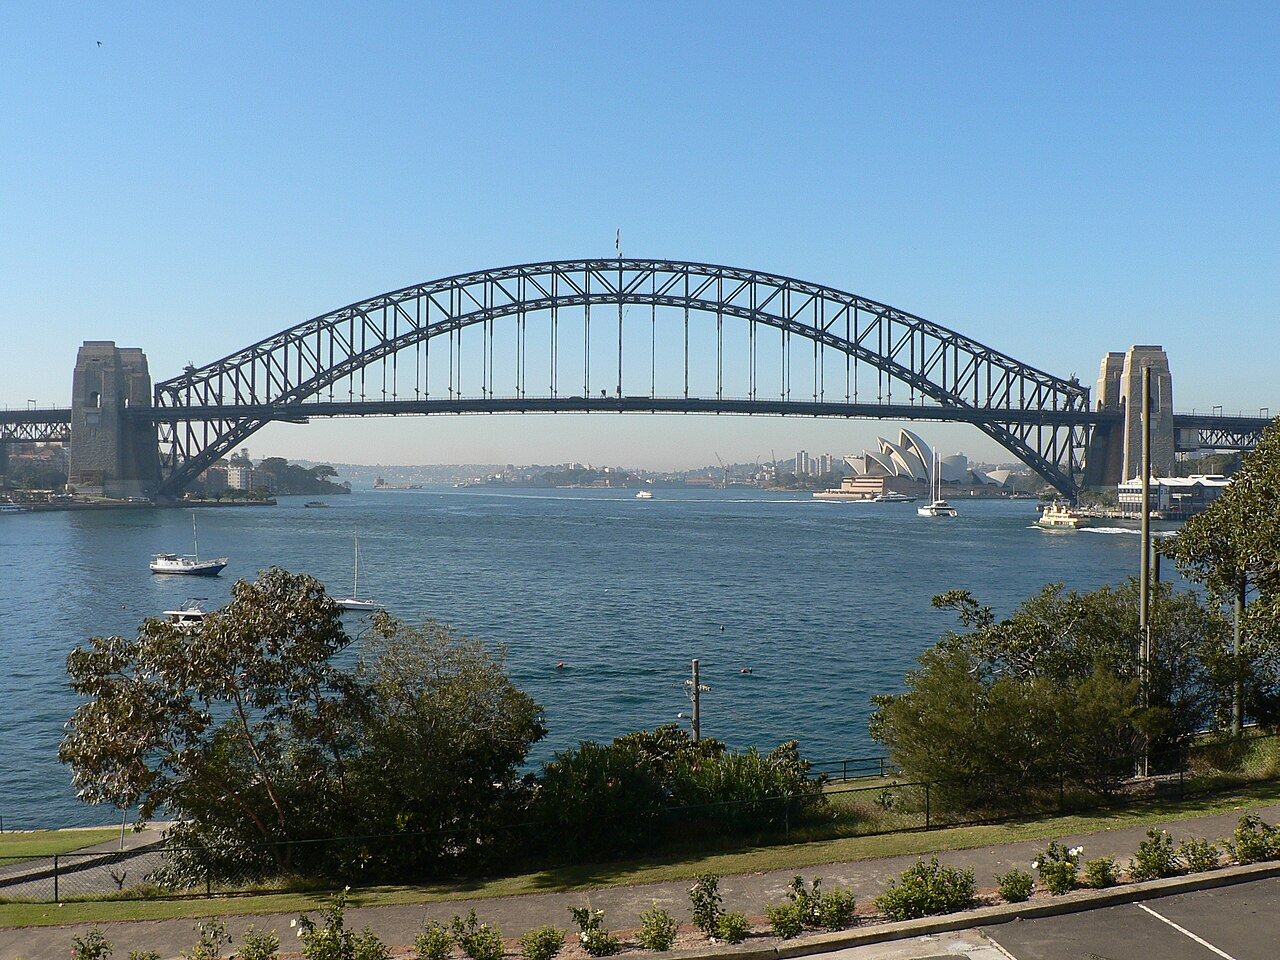
\includegraphics[width=\linewidth]{figures/Sydney-Harbour_bridge.JPG}
        \caption{Hafen Br\"ucke Sydney\parencite{rabich2023}}
    \end{minipage}
\end{figure}

Man sieht dies auch hier am Beispiel der ``Sydney Harbour Bridge'', diese wurde 
1932 fertig gestellt, gebaut mit reinen Berechnungen, ohne jegliche Hilfe von Algorithmen. 

Hier sehe ich eine Chance f\"ur diverse Algorithmen und Simulationen die einen
solchen Prozess erleichtern k\"onnten. Nicht nur Topologische Optimierungen aus
statischer Sicht, auch andere Simulationen um Strukturen z.B. unter extremen Wind 
Bedingungen auf Resonanz zu pr\"ufen.


\section{Beispiele f\"ur Verfahren und Baustoffe}
In den folgenden Sektionen werde ich mich aus Gestalterischer- und Produktionssicht mit
Verfahren und Baustoffen auseinandersetzen.

Die Institution von der ich hier die meisten Erkentnisse nehme ist die DART Michigan
(Digital Architecture Research \& Technologies), dies ist ein Kolleg der
Universit\"at Michigan, fokusiert auf Architektur-Forschung mit Schwerpunkt auf 
neue Baumaterialen und Parametrischem Design.

Selbst konnte ich in diesem Bereich keine Erfahrungen machen da alle ben\"otigten Maschienen 
ohne Ausnahme sehr teuer sind, wenn \"uberhaupt der \"Offentlichkeit zug\"anglich.

Eine andere gro\ss{}e Institution in dieser Forschung ist die Technische Uni M\"unchen,
diese ist aber meines Wissens nur in den Computionalen und Topologischen Aspekten 
des Designs besch\"aftigt.


\subsection{M\"ogliche Baustoffe / 3d-Druck in der Architektur}
Die Materialforschung ist wahrscheinlich eine immer present und interesante
Sparte der Wissenschaft, meiner Meinung nach vorallem die aktuellen Erkentnisse
der FDM Materialien f\"ur Bau sowie Produktdesign. Technologie macht es
m\"oglich alles von Plastik bis Beton, Sandstein und Holz zu drucken, was vor
wenigen Jahrzehnten undenkbar war, insbesondere der Gedanke das einige
Privatleute zuhause sich alles aus Plastik drucken k\"onnen was sie wollen
statt auf Hersteller Angewiesen sein zu m\"ussen.

Aus Zeit und Platgr\"unden kann ich im folgenden nur Beispiele verschiedener
Institutionen vorstellen statt eine geb\"uhrende Analyse zu den einzlnen
Bauwerken zu machen.

    \subsubsection{Beton}
    \begin{figure}[H]
        \centering
        \begin{minipage}{0.25\textwidth}
           \centering
           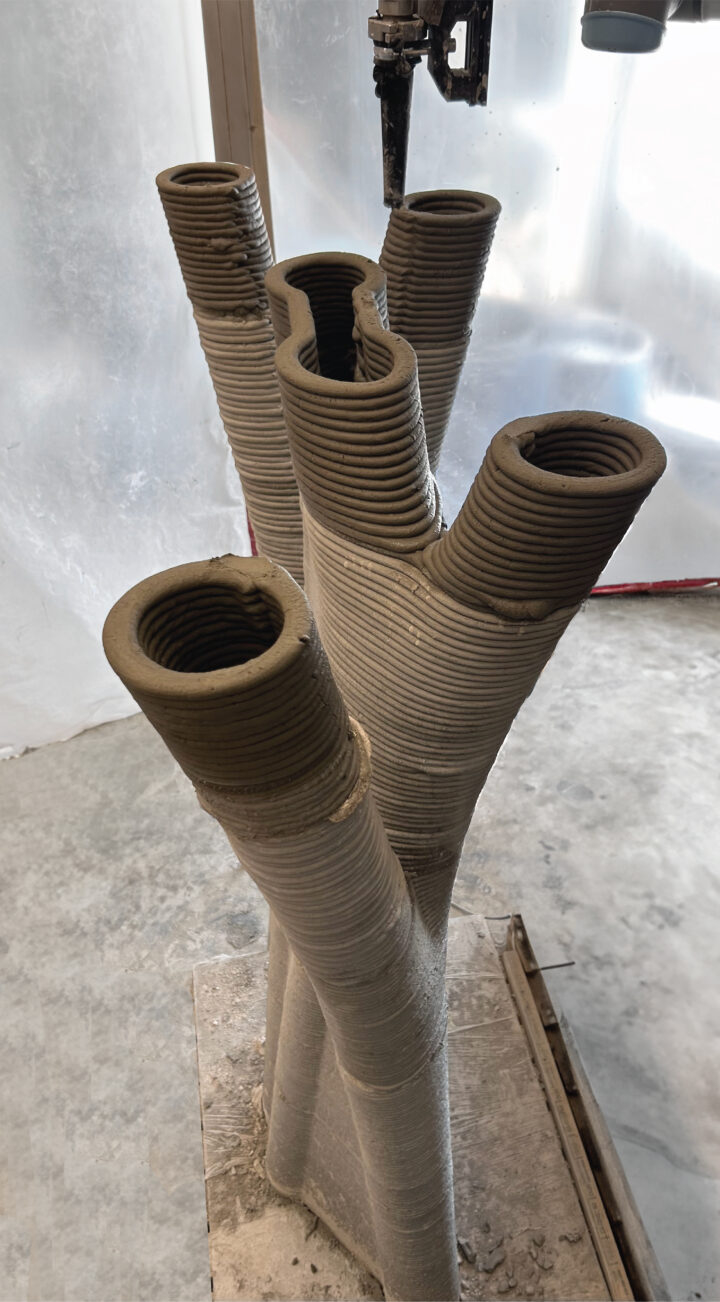
\includegraphics[width=\linewidth]{figures/beispiele/meibodi-2023-1.jpg}
           \caption{Gedruckte Betonstrucktur leer \parencite{meibodi2023}}
           \label{fig:leer}
        \end{minipage}
        \begin{minipage}{0.4\textwidth}
            Hier sieht man links Abbildung \ref{fig:leer}, in diesem Bild wurden gerade die oberen Schichten gedruckt.
            Auf der rechten Abbildung \ref{fig:voll} sieht man das
            Gedruckte einen Schritt weiter, der Beton wurde gef\"ullt und mit Stahl verst\"arkt.

            Aus diesem Beipiel kann man Ableiten was auf einem Gr\"o\ss{}erem Ma\ss{}stab mit richtigen 
            Maschienen machen kann, Ich sehe hier einen Weg wie man z.B. Rohbau f\"ur H\"auser mit diesem 
            Verfahren machen kann.
        \end{minipage}
        \begin{minipage}{0.25\textwidth}
           \centering
           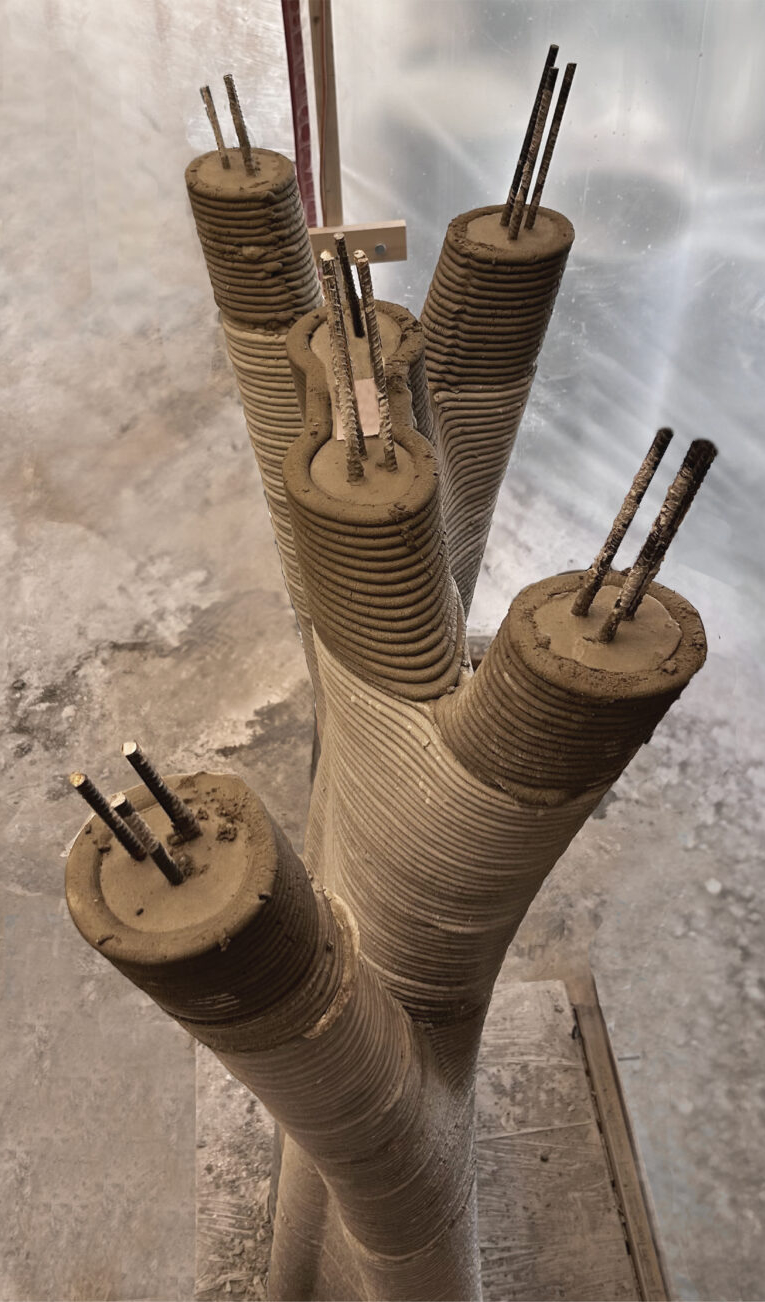
\includegraphics[width=\linewidth]{figures/beispiele/meibodi-2023-2.jpg}
           \caption{Gedruckte Betonstrucktur gef\"ullt \parencite{meibodi2023}}
           \label{fig:voll}
        \end{minipage}
    \end{figure}

Mitlerweile ist der FDM-Druck nichtmehr in Frage nach M\"oglichkeit, sondern im entstehen als valides
Werkzeug in der Bauindustrie, zur Zeit sind es
``Starchitekten\footnote{Ber\"uhmte Architekten, die sich mehr trauen k\"onnen.}'' aber ich gehe stark 
davon aus das wir 3d-Druck immer mehr im Bau sehen werden in der Zukunft wir sind noch viele Jahre davon 
entfernt das es ``normal'' ist, aber diese Zeit wird kommen.

\subsubsection{Pflanzenfasern}
Mit Pflanzenfasern kann man noch keine H\"auser bauen aber denoch m\"ochte ich hier ein Verfahren erw\"ahnen
das die Bauindustrie unerst\"utzt, die folgende Forschung ist aus der oben erw\"ahnten DART Institution \parencite{kahn2023}.

Eine Akteurin in der Parametrischen Architektur war Zaha Hadid mit einem
ihrer Werke werde ich mich in der Sektion \ref{sec:hadid}
auseinandersetzen, f\"ur jetzt mit den Bauweisen des Ph\ae{}nos Wolfsburg
um diese in Kontrast zu setzen mit einer anderen neu-entwickelten L\"osung 
der DART \parencite{kahn2023}.
    \begin{figure}[H]
        \begin{minipage}{0.4\textwidth}
           \centering
           \vfill
           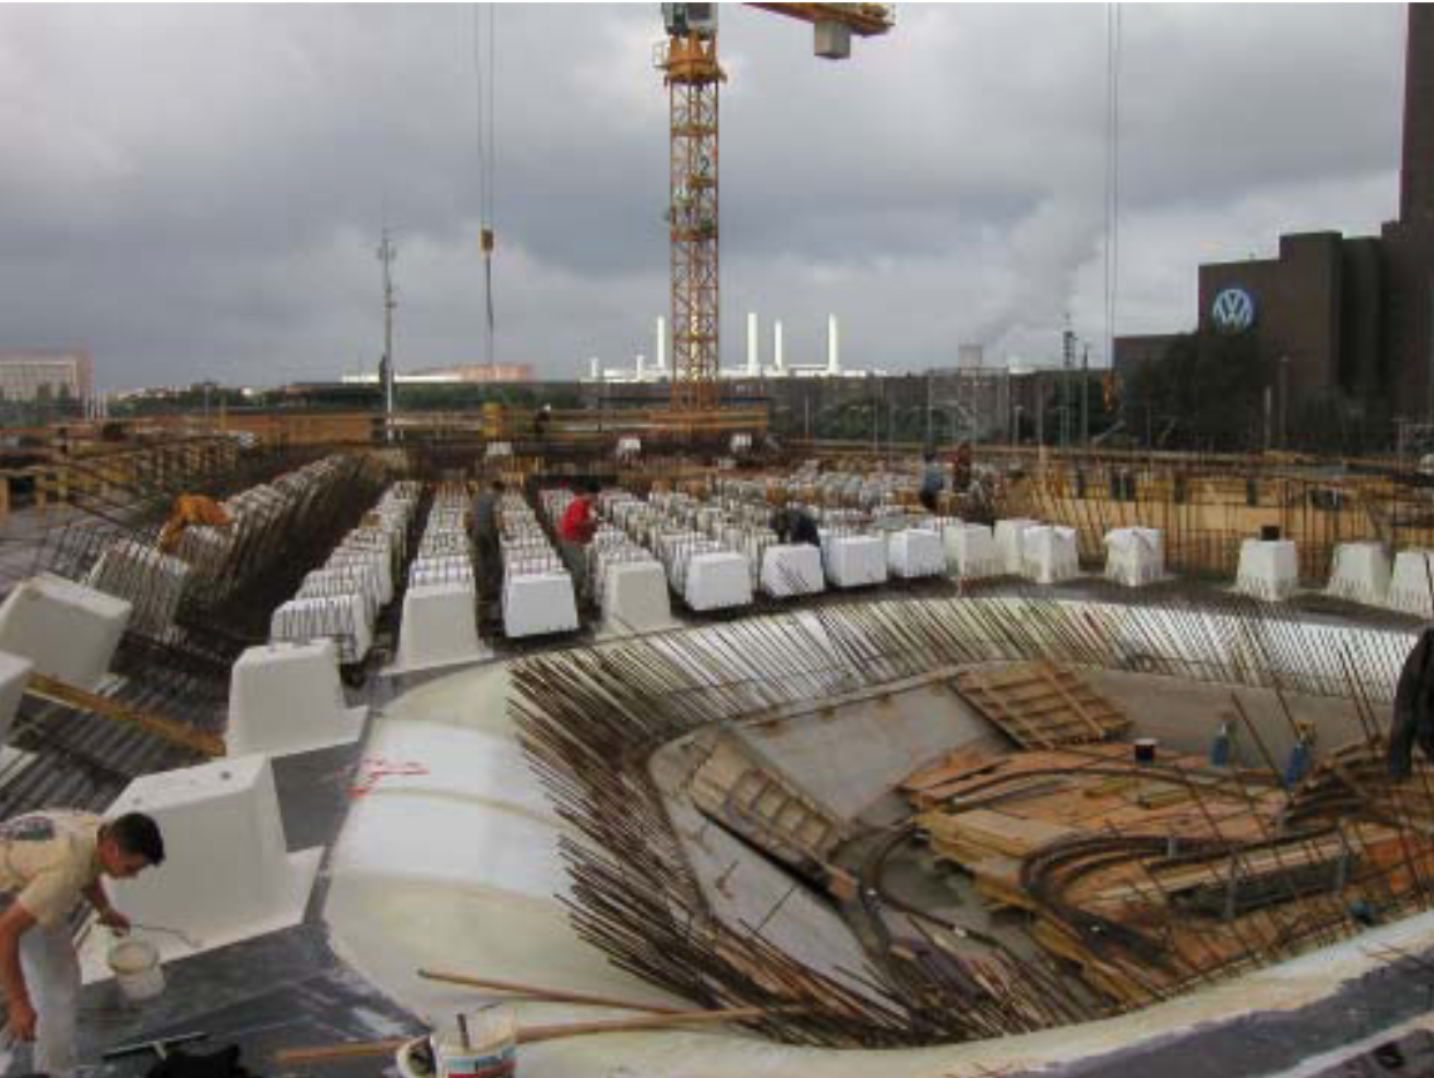
\includegraphics[width=\linewidth]{figures/beispiele/phaeno-307-1.png}
           \caption{Ph\ae{}no Bau \parencite{mayer}}
           \label{fig:bau-phae-1}
        \end{minipage}
            \hfill
        \begin{minipage}{0.4\textwidth}
           \centering
           \vfill
           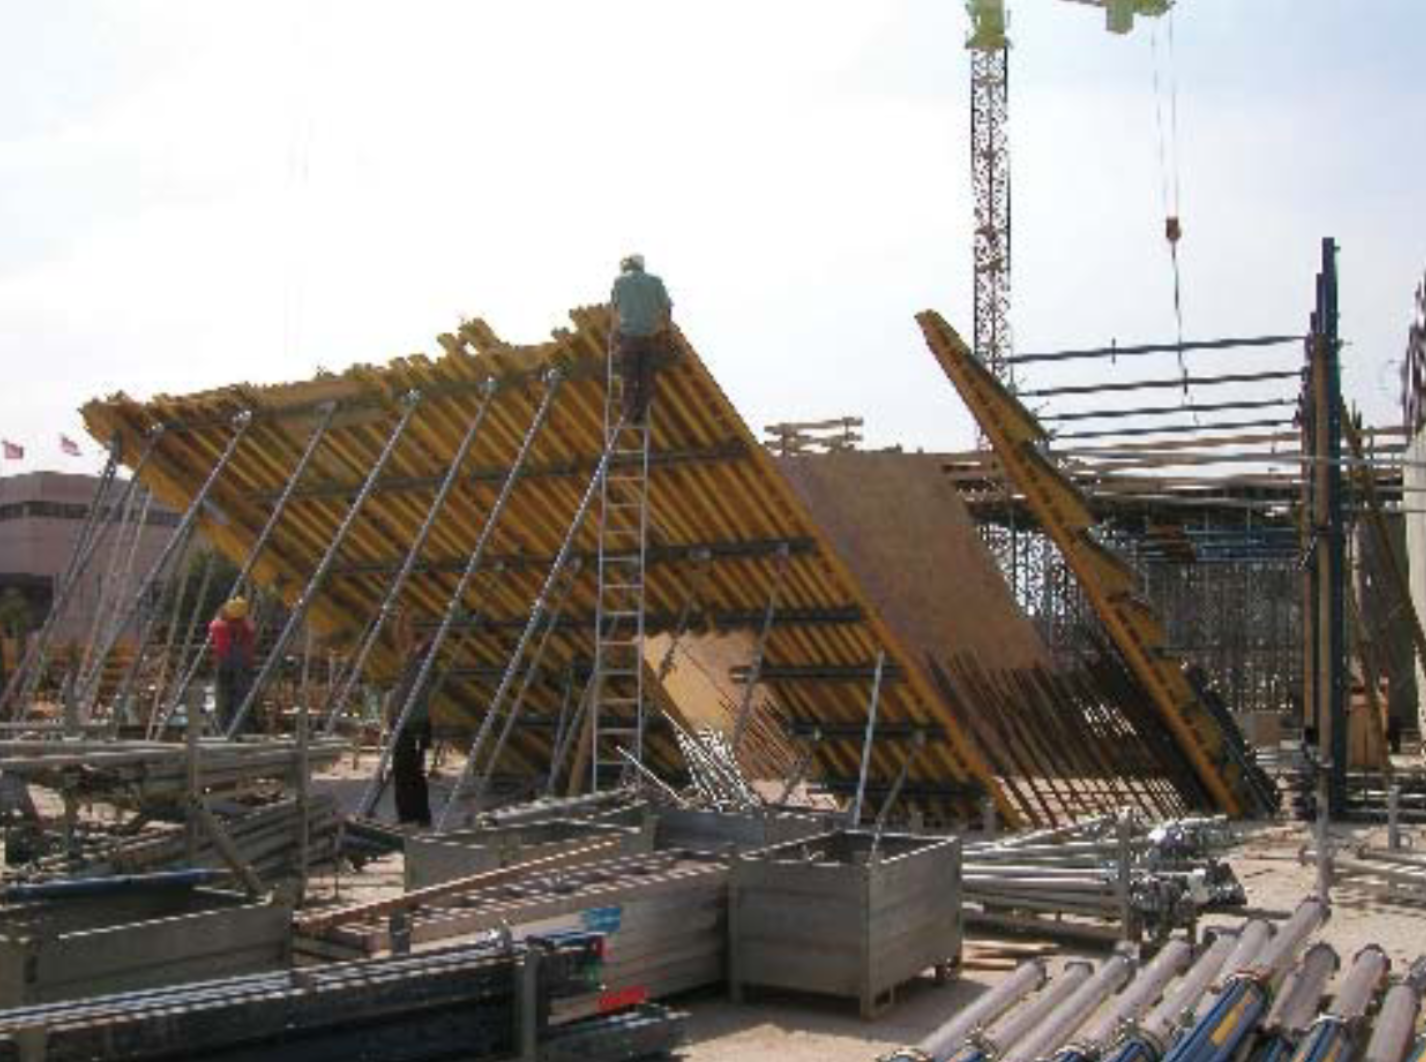
\includegraphics[width=\linewidth]{figures/beispiele/phaeno-307-2.png}
           \caption{Ph\ae{}no Bau \parencite{mayer}}
           \label{fig:bau-phae-2}
        \end{minipage}
    \end{figure}

    Hier in den Abbildungen \ref{fig:bau-phae-1} \& \ref{fig:bau-phae-2}
    sieht man die Verwendung von unmengen an Plastik, Holzplanken die verst\"arkt 
    werden m\"ussen und vielem weiterem. Vor einem Jahr besch\"aftigte ich mich im Rahmen
    einer anderen Ausarbeitung unter anderem mit diesem Bauwerk und wunderte mich 
    \"uber die nahezu verschwenderische Verwendung von Plastik. Wie es \parencite{mayer} in 
    dem Titel eines Fachartikels des ``Expertenforum Beton'' gut sagt:
    ``SCC\footnote{SCC: Selbstverdichtender Beton der diese Verfahren
    m\"oglich macht.} als Antwort auf die Herausforderung architektonischer
    Wunschvorstellungen''. Diese Aussage der Betonexperten sagt mir das
    diese nichtmehr \"uberlegen ob etwas m\"oglich ist, sondern eher davon
    aussgehen k\"onnen das alles was man sich selbst oder ein Architekt vorstellen
    kann m\"oglich ist mit den neusten Verfahren.

    Dies bekr\"aftigt auch die DART Forschung zu Druckbarem Holz, bzw.
    Pflanzenfasern im Allgemeinen. Diese ist n\"amlich darauf gekommen,
    dass man durch Druck von Organischem Material eine Form f\"ur Giesbeton
    machen k\"onnte welche Kompostierbar ist und den M\"ull der
    Normalerweise entstehen w\"urde nahezu abl\"ost und das Giesen von SCC
    weniger bis auf den Beton an sich kaum bedenklich macht.

    \begin{figure}[H]
        \begin{minipage}{0.4\textwidth}
           \centering
           \vfill
           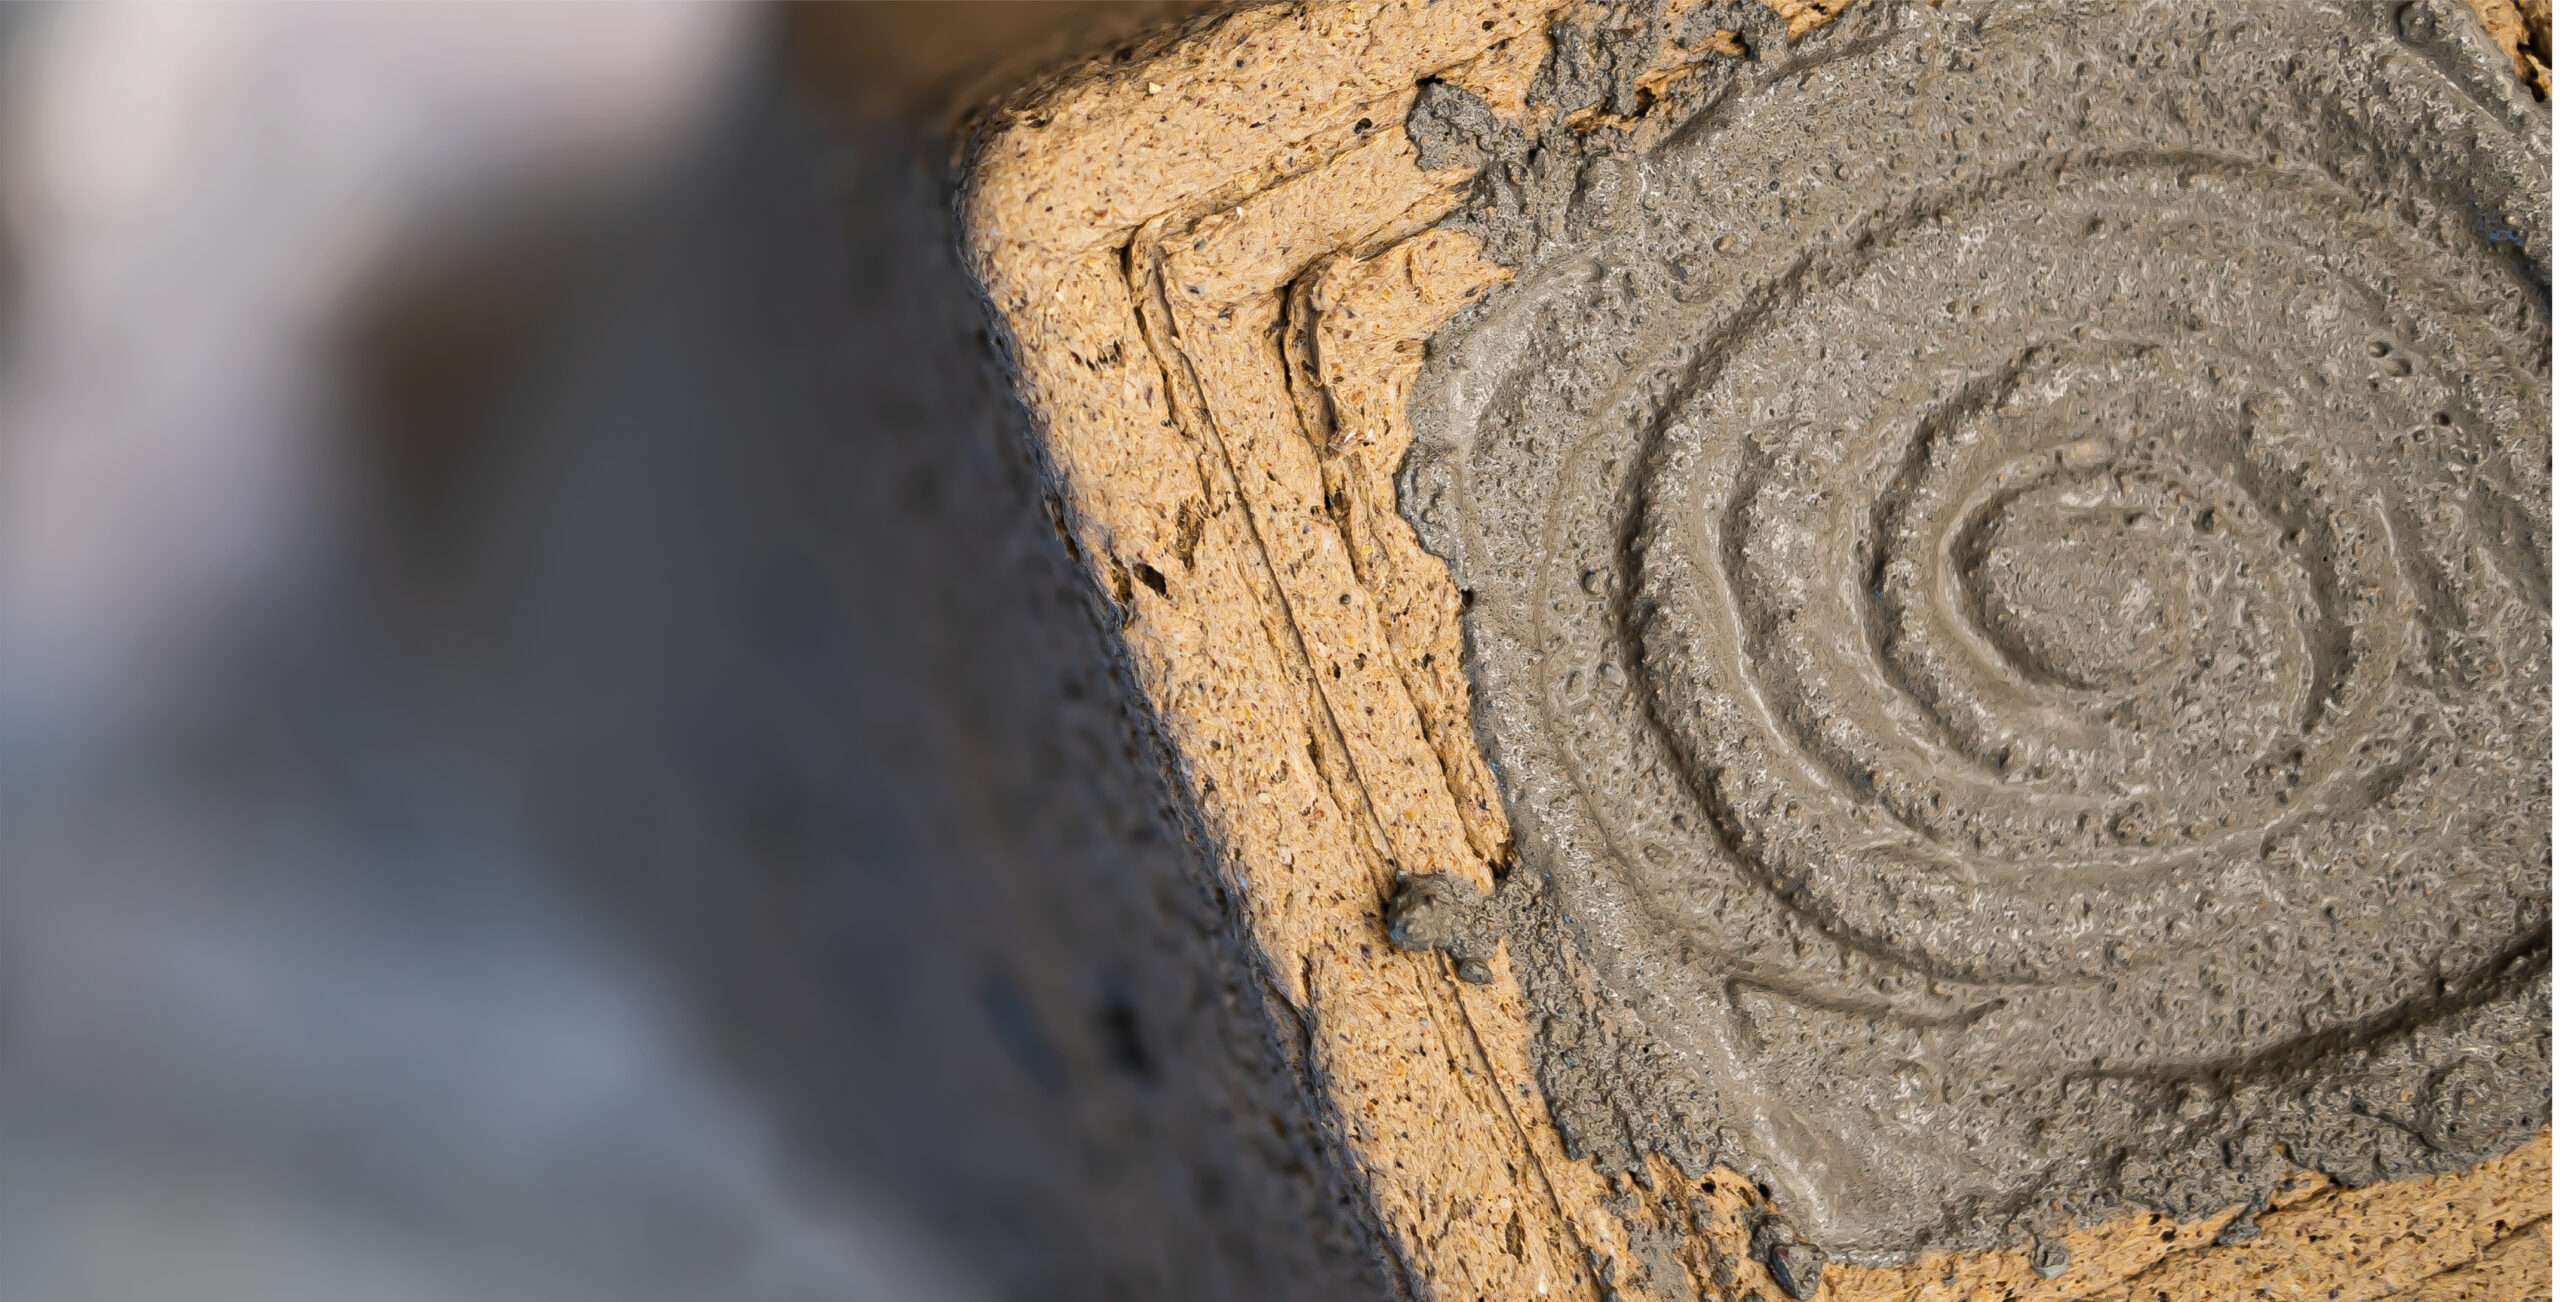
\includegraphics[width=\linewidth]{figures/beispiele/kahn-2023-1.jpg}
           \caption{\parencite{kahn2023}}
           \label{fig:kahn-1}
        \end{minipage}
            \hfill
        \begin{minipage}{0.4\textwidth}
           \centering
           \vfill
           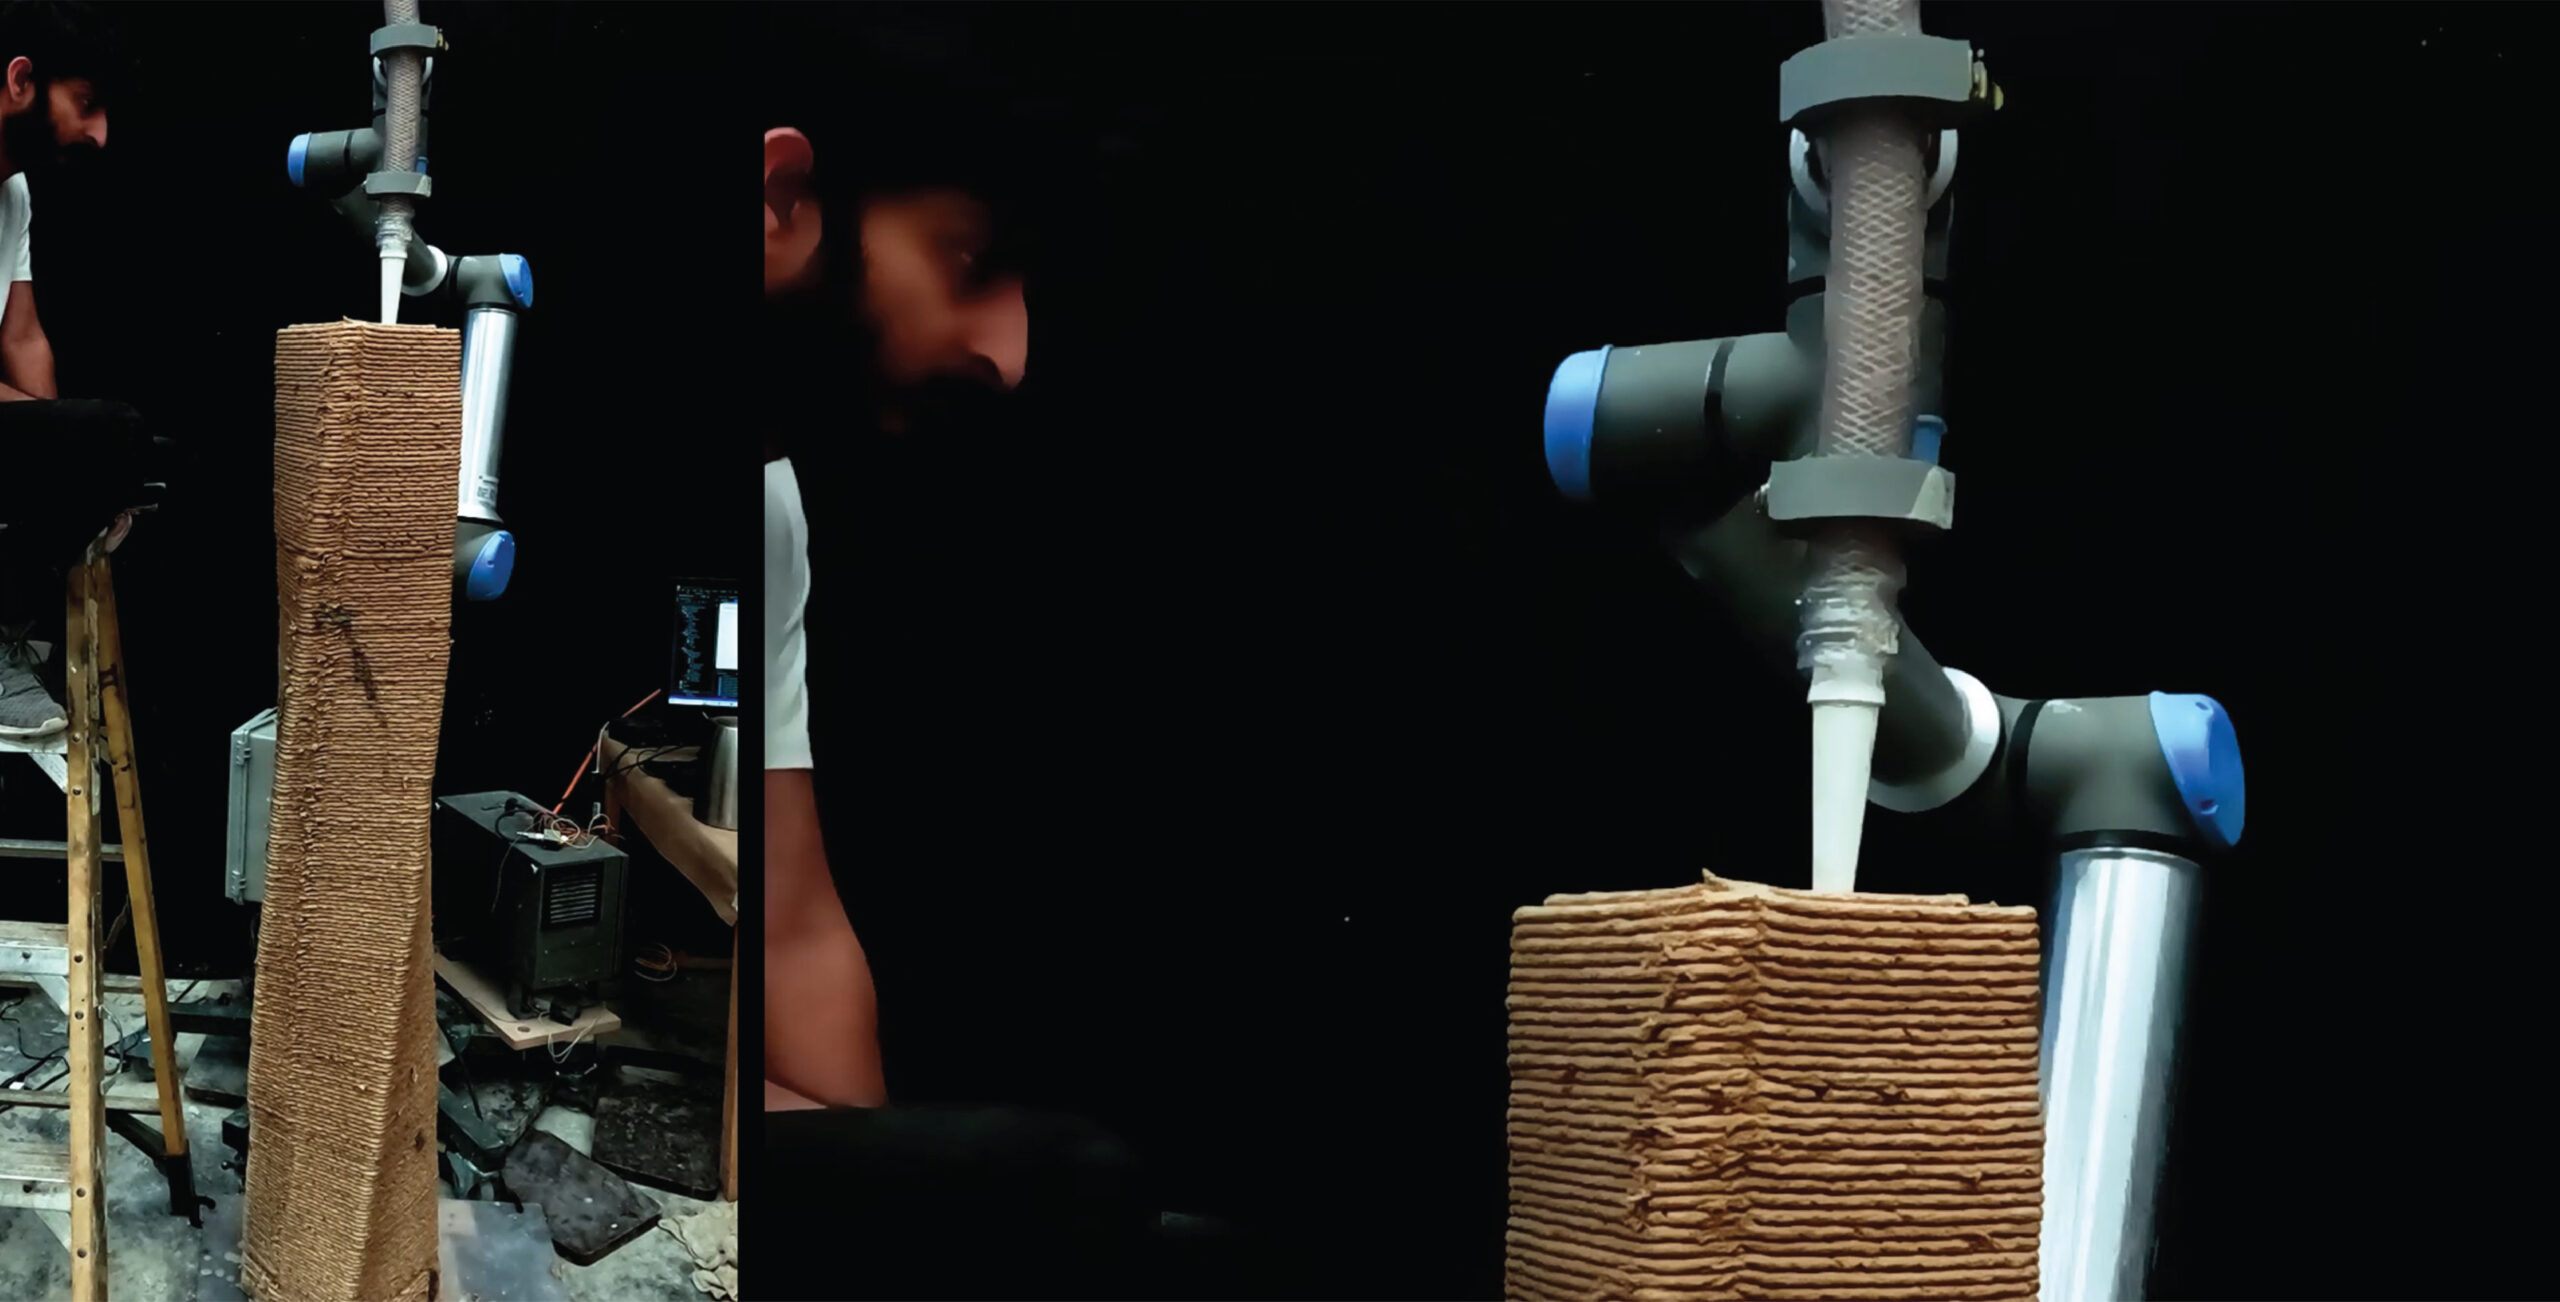
\includegraphics[width=\linewidth]{figures/beispiele/kahn-2023-2.jpg}
       \caption{\parencite{kahn2023}}
           \label{fig:kahn-2}
        \end{minipage}
    \end{figure}



\subsection{FDM-Druck f\"ur Produktdesign}
Der FDM\footnote{Fused Deposit Modeling}-Druck hat sich im letzten Jahrzehnt gut im
Produktdesign etabliert, weniger zum erstellen von Produkten aber als essentielles 
Werkzeug beim Prototyping. Da der Designprozess fast 100\% digital l\"auft kann man 
sich einfach den aktuellen Stand des Projektes ausdrucken. Die Drucker werden auch 
f\"ur Privatpersonen und z.B. Studenten immer Leistbarer Teils Drucker guter qualit\"at f\"ur
unter 300€.


\section{Beispiele im Produktdesign}

    \subsection{St\"uhle}
    Es gibt einige Topologisch optimierte St\"uhle, hier werde ich den von
    Joris Laarman \parencite{laarman2006} nehmen da dieser der erste war (erstmals 
    hergestellt 2006).
        \begin{figure}[H]
            \begin{minipage}{0.5\textwidth}
               \centering
               \vfill
               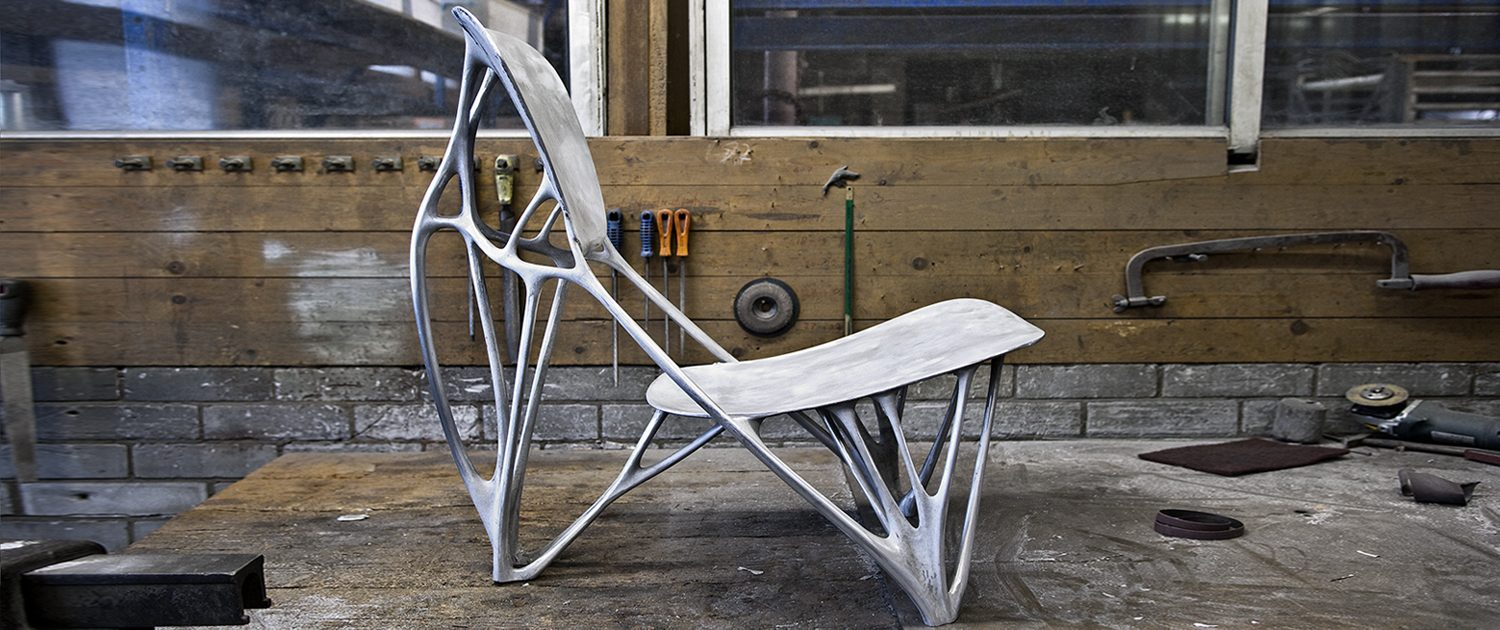
\includegraphics[width=\linewidth]{figures/beispiele/stals-2.jpg}
               \caption{Bone Chair \parencite{laarman2006}}
               \label{fig:stuhl-1}
            \end{minipage}
                \hfill
            \begin{minipage}{0.3\textwidth}
               \centering
               \vfill
               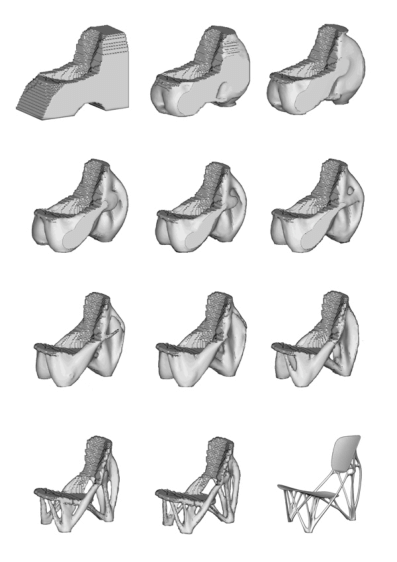
\includegraphics[width=\linewidth]{figures/beispiele/stals-1.png}
               \caption{Iterative Berechnung. \parencite{stals2015}}
               \label{fig:stuhl-2}
            \end{minipage}
        \end{figure}

        Hier sieht man zum einen gut das organisch-knochenartige Design des Stuhl links in Abb. \ref{fig:stuhl-1},
        zum anderen den iterativen prozess des topologischen Algorithmus, der
        mit den gegebenen Fl\"achen, Au\ss{}enbegrenzungen und Kr\"aften nach und nach den Stuhl rendert.
    

    \subsection{Beispiele des Ingeneurswesens}
    Beim h\"oren von minimalem Material und Maximaler St\"arke denkt man an das
    Ingeneurswesen. Diese haben auch einen Gro\ss{}en nuzten von der Erkentniss aus 
    der topologischen Forschung mit Stahl als einfach bearbeibarem Werkstoff.

    Ich werde nicht tief auf diese Verwendung eingehen aber einzelne Bilder zur 
    Veranschauung und aus Forschung von Firmen erw\"ahnen. 


    \begin{figure}[H]
        \begin{minipage}{0.4\textwidth}
           \centering
           \vfill
           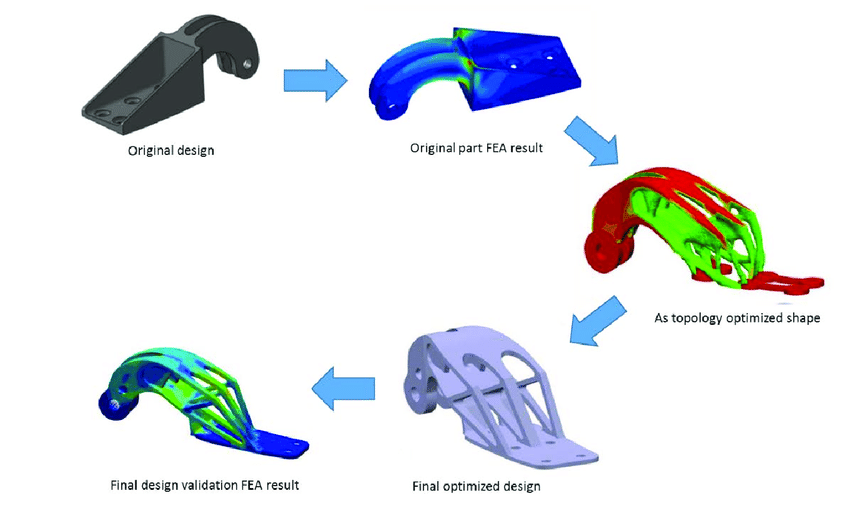
\includegraphics[width=\linewidth]{figures/beispiele/gebisa-topo-workflow.png}
           \caption{Workflow mit Parametrischem Design \parencite{gebisa2017}.}
           \label{fig:ing-1}
        \end{minipage}
            \hfill
        \begin{minipage}{0.4\textwidth}
           \centering
           \vfill
           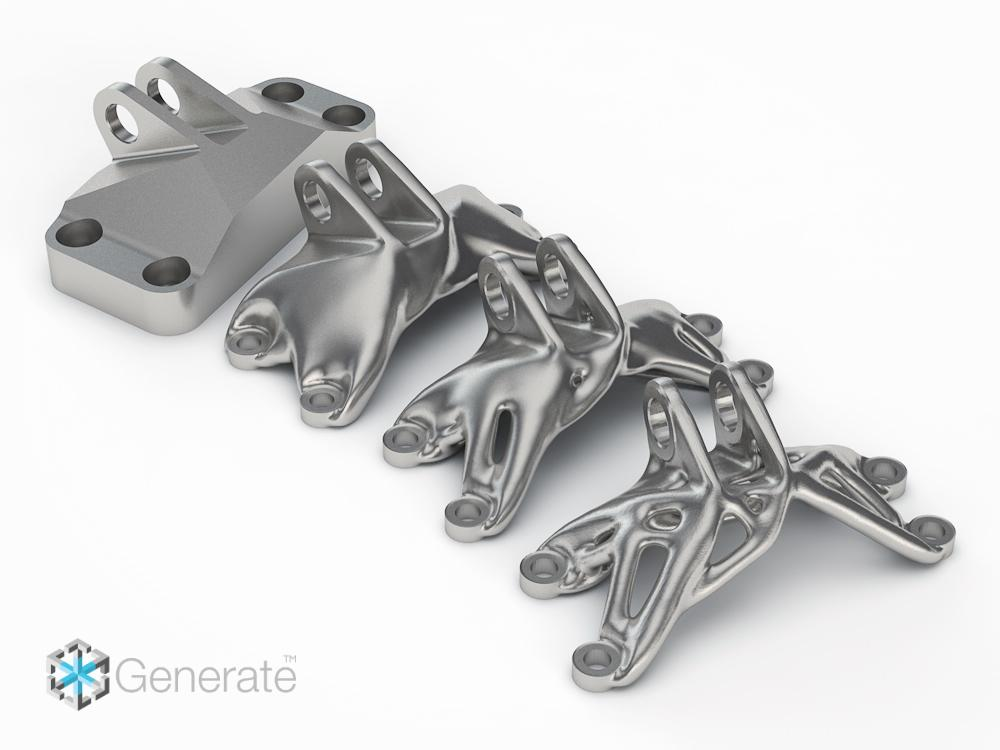
\includegraphics[width=\linewidth]{figures/beispiele/topo-ingeneur-2.jpg}
           \caption{Iterative Berechnung.}
           \label{fig:ing-2}
        \end{minipage}
    \end{figure}

%%%%%%%%% hier infos anf\"ugen

\section{Beispiele in der Architektur}

    \subsection{Zaha Hadid}

    Wenn man \"uber Parametrisches Design in der Architektur nachdenkt und ansatzweise Architektur 
    interessiert ist f\"allt einem wahrscheinlich direkt Zaha Hadid ein.

    Sie war die Architektin des Parametrisches Design, von ende der 70 Jahre bis nach 
    Ihrem Tod 2016 war Sie essentiell f\"ur den Parametrie eigenen Stil. Man kann noch nicht sagen 
    wie gro\ss{} ihr Einfluss in der Architektur ist, aber definitiv beachtlich.

    In ihren Werken ist der fokus der Parametrie aber nicht auf z.B. Topologie, sondern eher auf 
    kontinuierliche Linien wie in Abbildung \ref{fig:hadid-1} oder
    Kubismus-artige gebilde wie in Abbildung \ref{fig:hadid-2}.


    \label{sec:hadid}
    \begin{figure}[H]
        \begin{minipage}{0.4\textwidth}
           \centering
           \vfill
           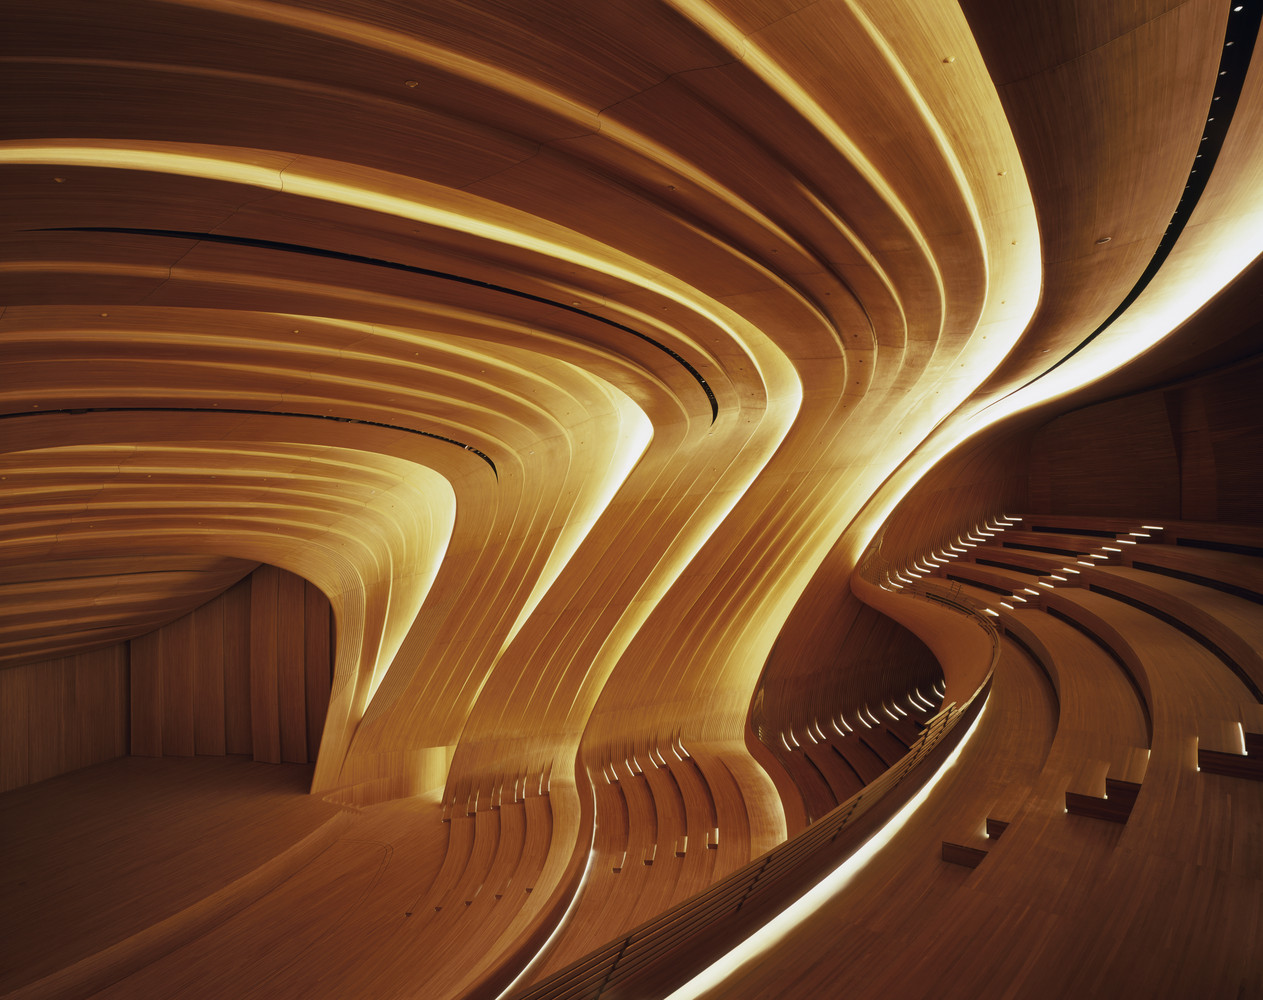
\includegraphics[width=\linewidth]{figures/beispiele/architektur/hyder-aliyev-hadid.jpg}
           \caption{Hyder Aliyev Center Azerbaijan}
           \label{fig:hadid-1}
        \end{minipage}
            \hfill
        \begin{minipage}{0.4\textwidth}
           \centering
           \vfill
           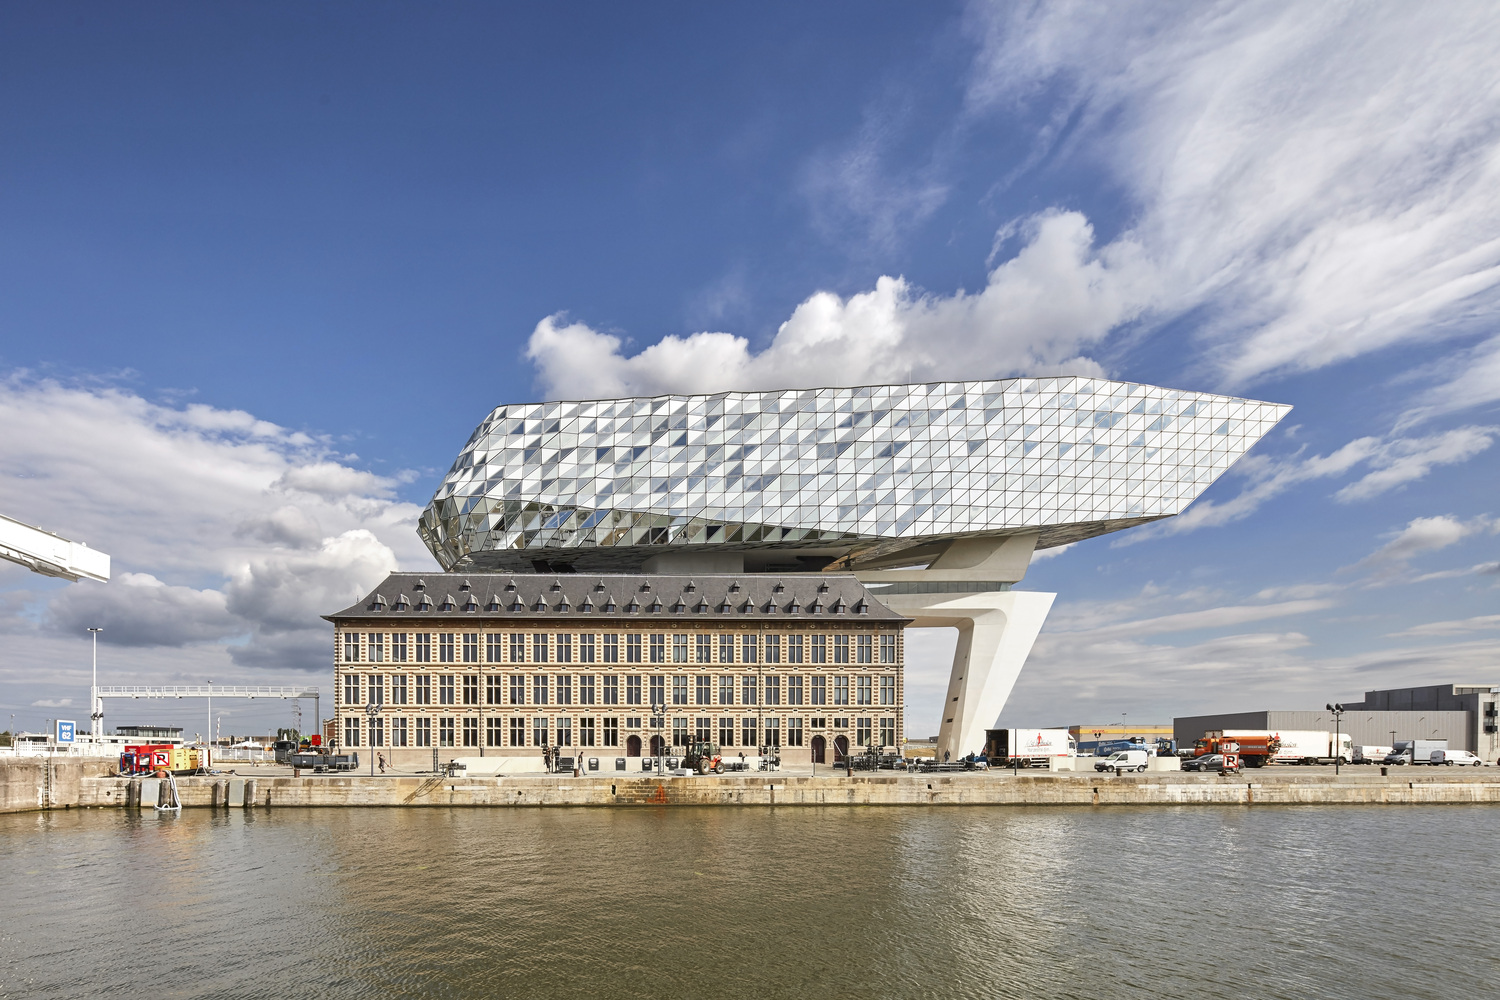
\includegraphics[width=\linewidth]{figures/beispiele/architektur/antwep-port-house.jpg}
           \caption{Port House Antwerp}
           \label{fig:hadid-2}
        \end{minipage}
    \end{figure}



\fakesection{Topologische Optimierung Tutorial in Solidworks}
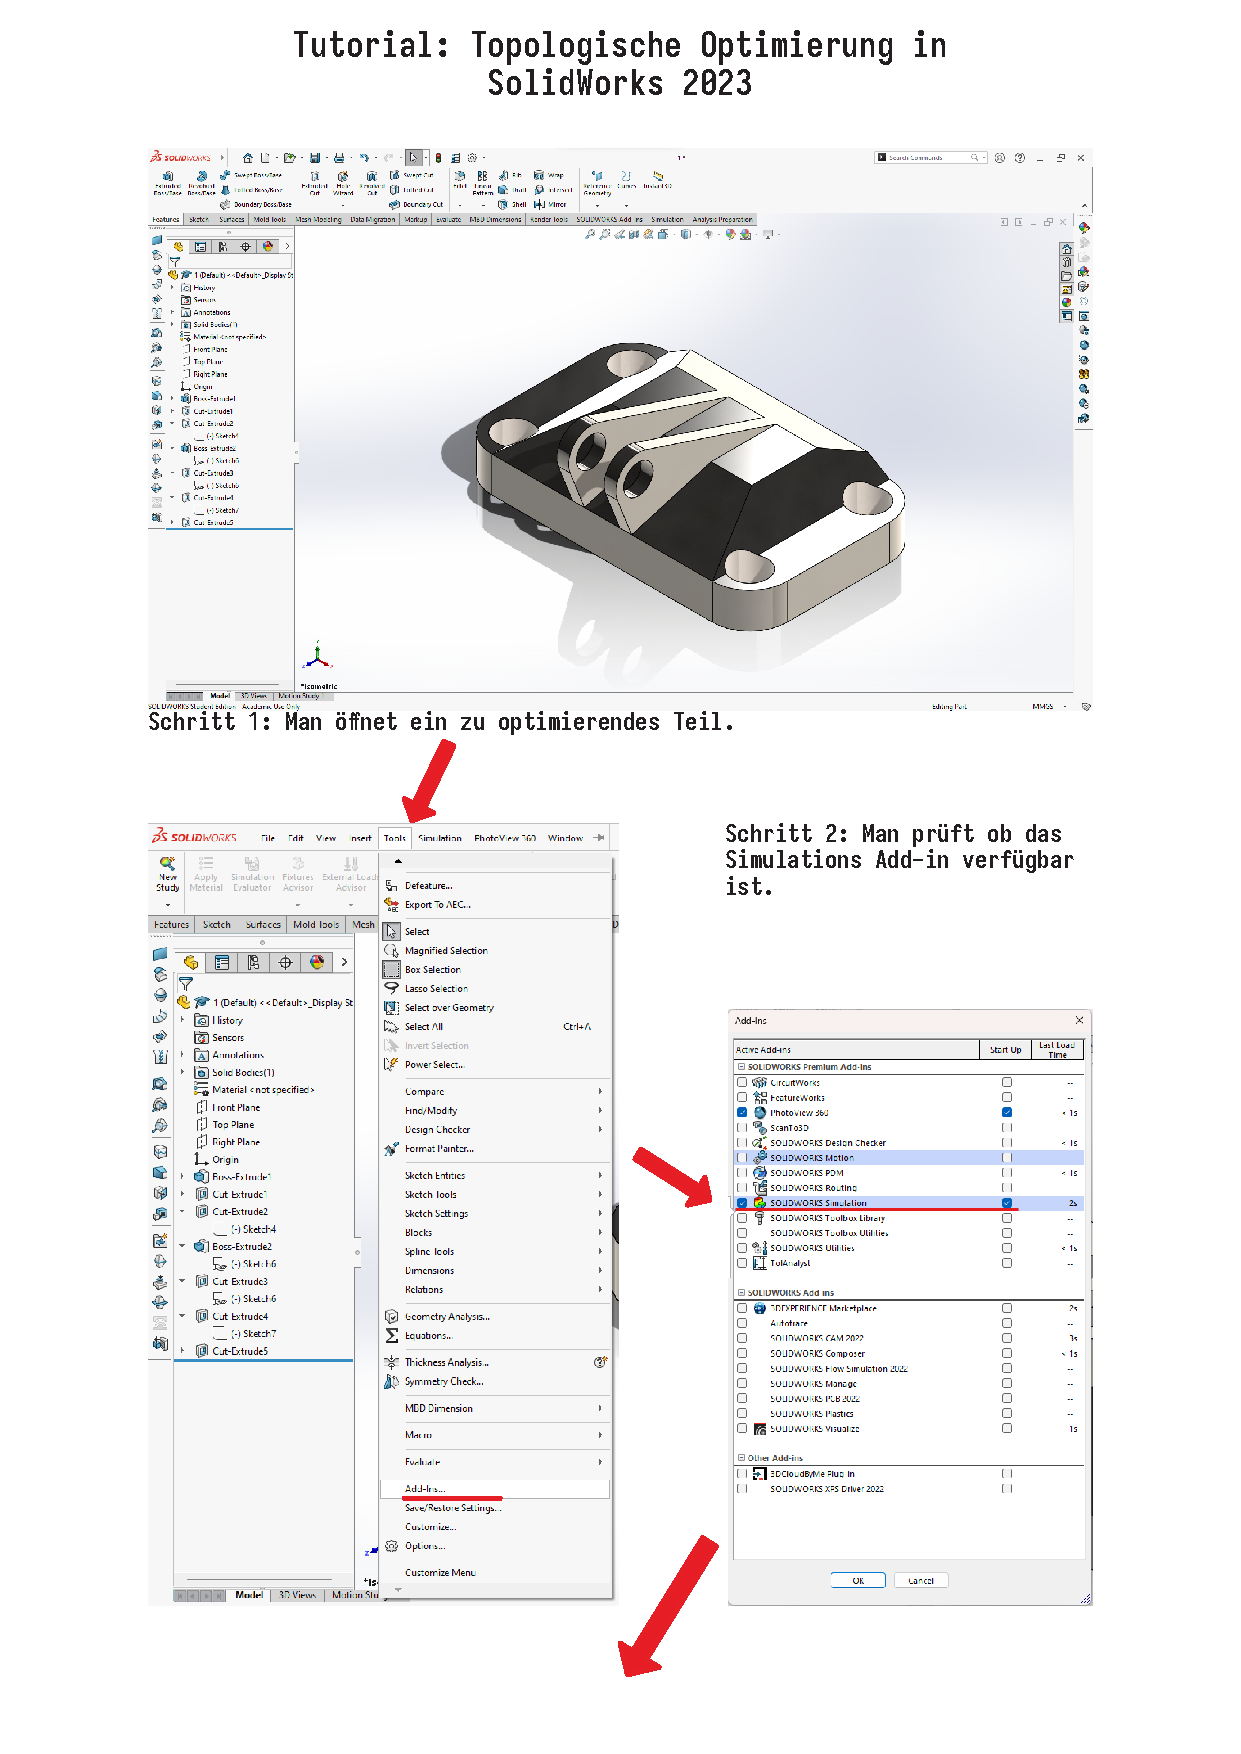
\includepdf[pages=-]{tutorial.pdf}
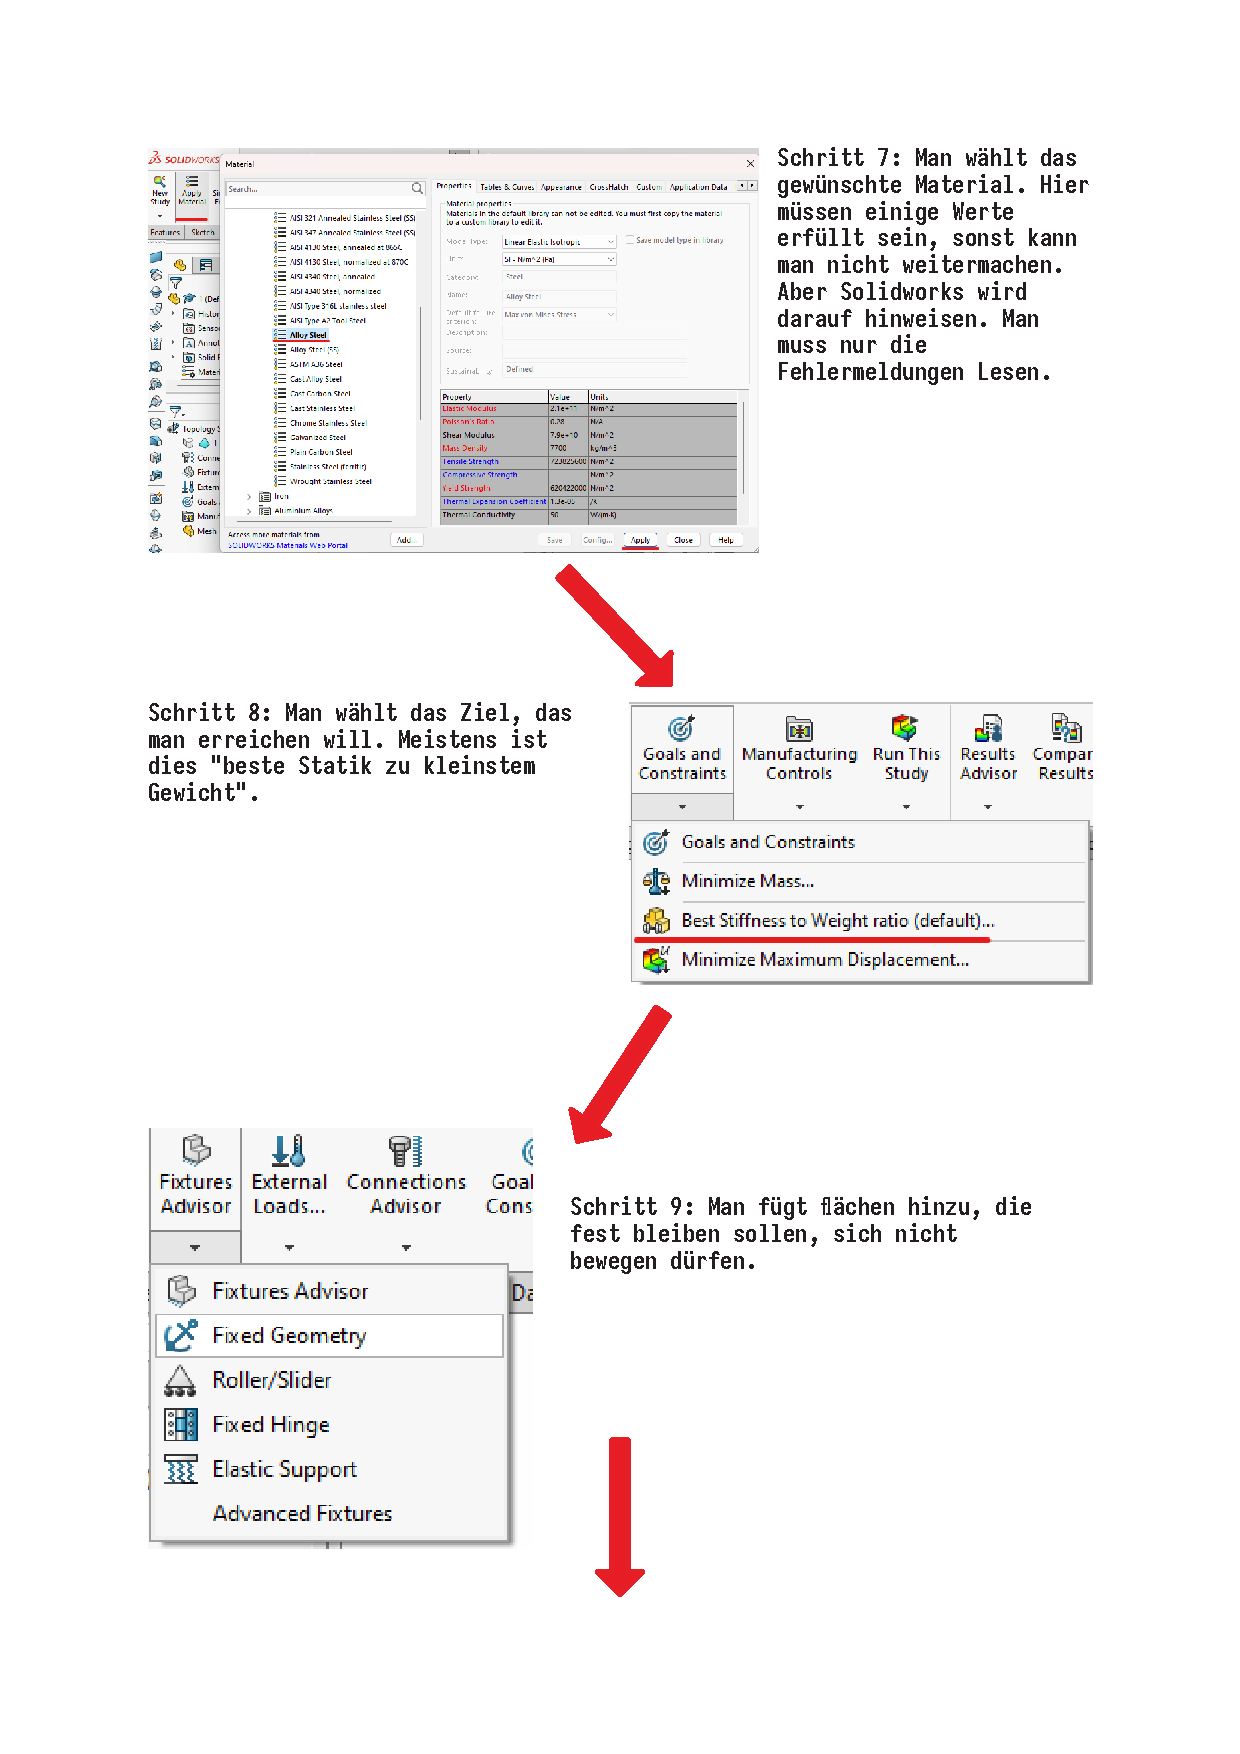
\includepdf[pages=-]{tutorial2.pdf}
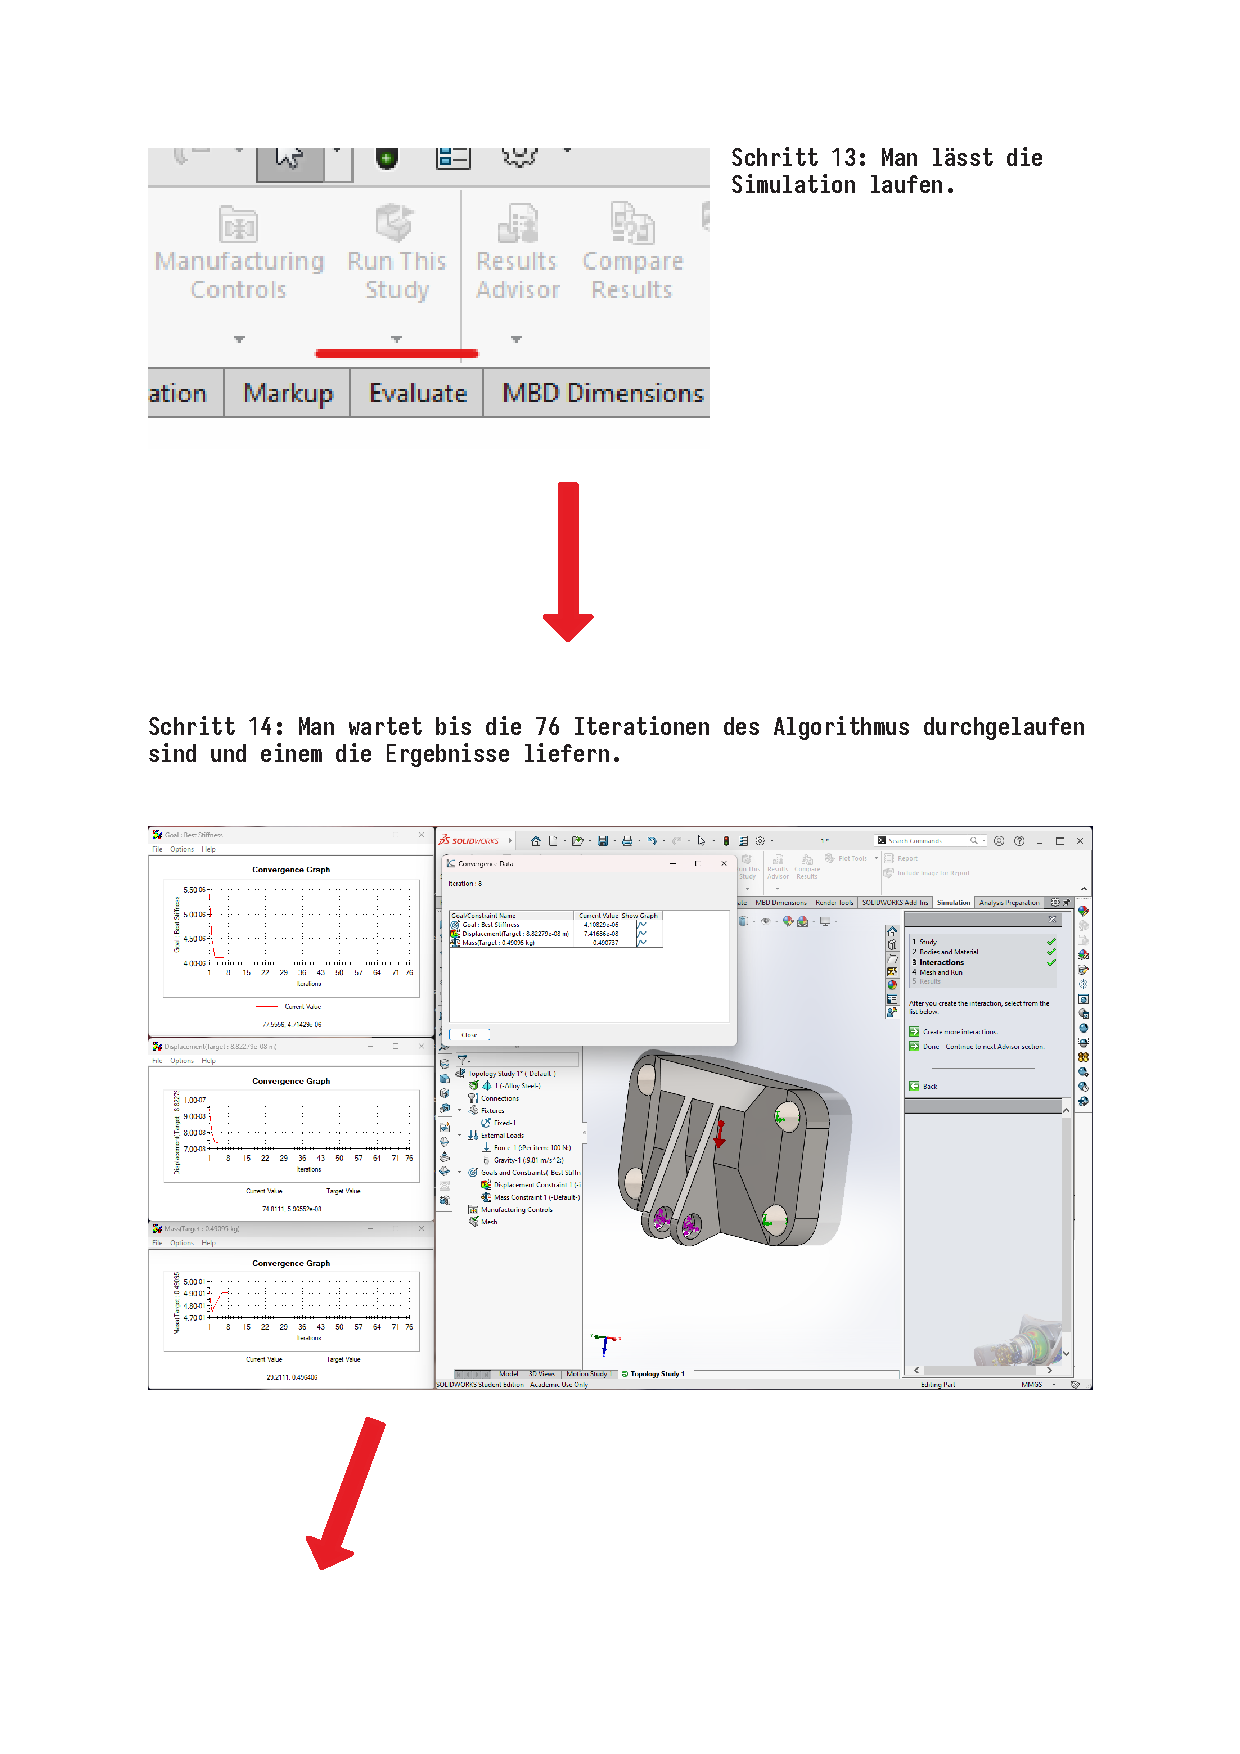
\includepdf[pages=-]{tutorial3.pdf}



\section{Andere CAD-Programme f\"ur Topologie}

    \subsection{RhinoCAD}
    RhinoCAD bietet viele M\"oglichkeiten f\"ur Parametrisches Design, vorallem
    mit der ``Grasshopper'' Extension. Dort hat man Blender-artige Nodes um
    Komplexe Funktionen und Strukturen zu erstellen.

    Es hat eine weitaus gr\"o\ss{}ere Eintrittsbariere als viele andere Software wie 
    Solidworks oder Fusion, ist aber kostenlos und am funktionalsten f\"ur das 
    Parametrische designen.

    \begin{figure}[htpb]
        \centering
        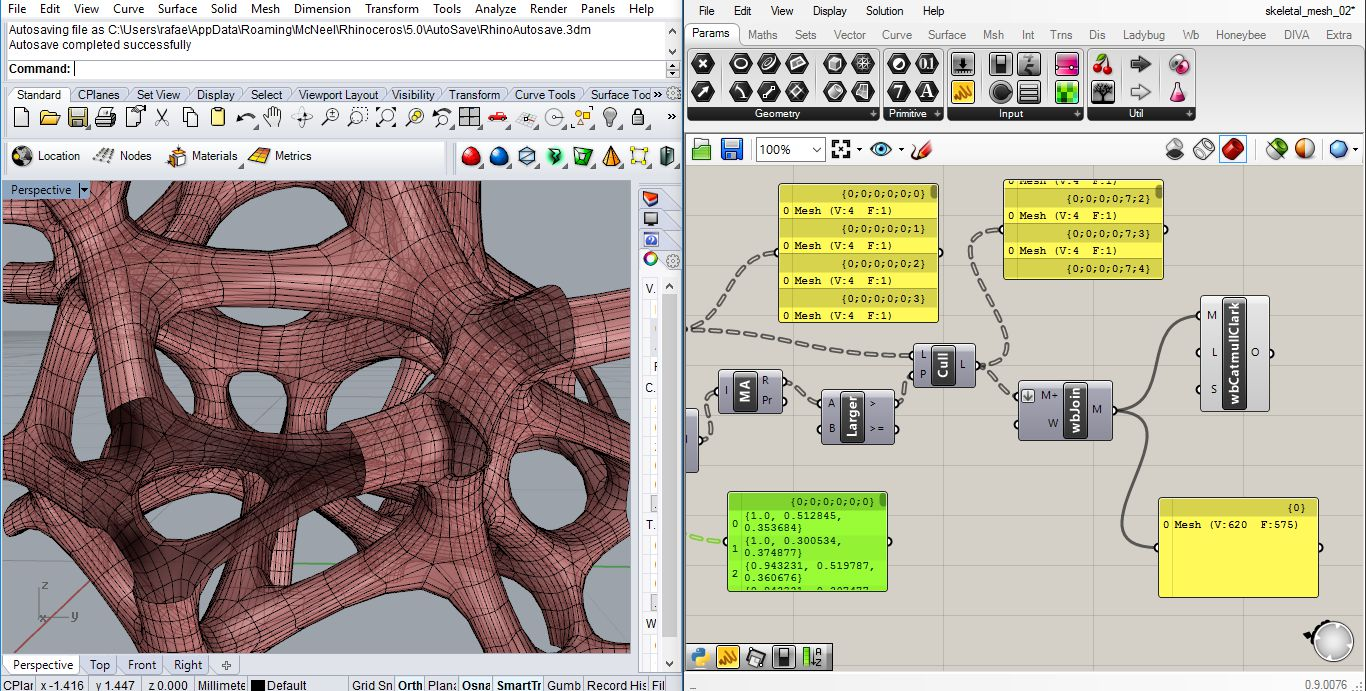
\includegraphics[width=0.8\textwidth]{figures/software/rhino.jpg}
        \caption{RhinoCAD Beispiel}
        \label{fig:rhino}
    \end{figure}

    \subsection{Fusion360}
    Fusion360 ist ein sehr beliebtes Programm im Hobby-Bereich, hat aber viele 
    Punkte die es mir nicht sinnvoll erscheinen lassen es in einer Professionellen 
    Umgebung zu nutzen.

    Z.B. kann man Analysen nicht selbst simulieren, und ohne Sch\"ulerlizens kosten diese
    um die 3 Euro pro St\"uck. Das ist sehr \"argerlich wenn man selbst einen Rechenintensiven
    Compute hat, aber im generellen mit jedem modernen Computer sollte dies zu rechnen kein
    Problem sein.

    Der essentielle Vorteil von Fusion360 gegen\"uber SolidWorks ist, dass es f\"ur Privatpersonen
    kostenlos ist, wenn auch sehr eingeschr\"ankt.

    \begin{figure}[H]
        \centering
        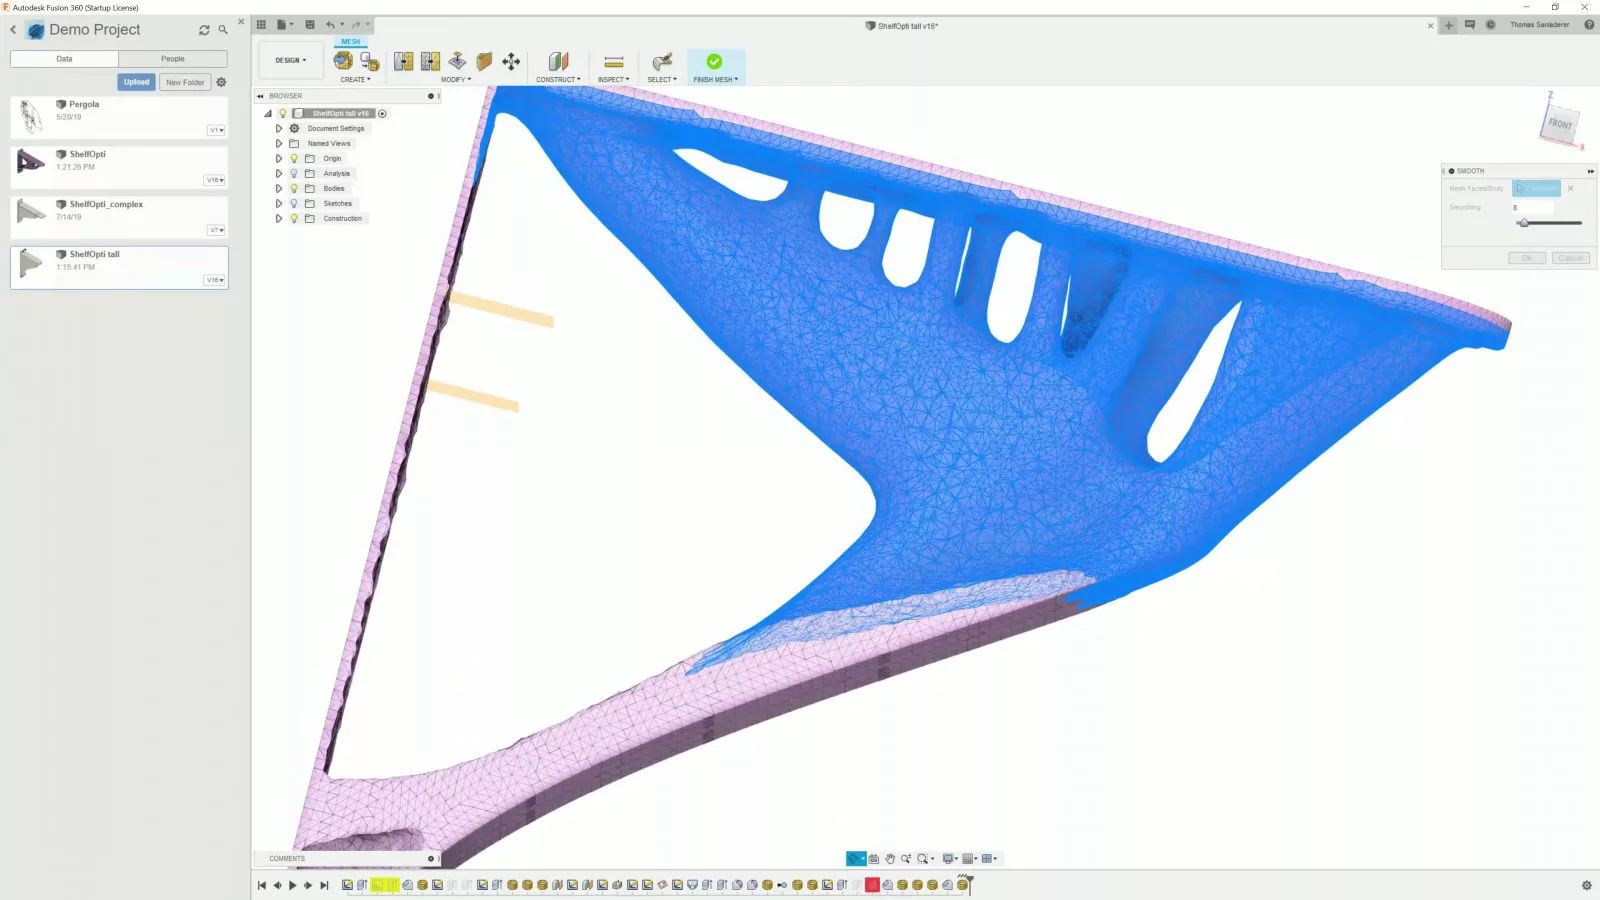
\includegraphics[width=0.8\textwidth]{figures/software/fusion.jpg}
        \caption{Fusion360 Beispiel}
        \label{fig:fusion}
    \end{figure}













%%%%%%%%%%%%%%%%%%%%%%%%%%%%%%%%%%%%%%%%%%%%%%%%%%%%%%%%%
%%%%%%%%%%%%%%%%%%%%% Bibliographie %%%%%%%%%%%%%%%%%%%%%
%%%%%%%%%%%%%%%%%%%%%%%%%%%%%%%%%%%%%%%%%%%%%%%%%%%%%%%%%

\newpage
\section{Empfohlene Literatur}
Die folgende Literatur kann ich für vertiefte Studien empfehlen.
\begin{itemize}
    \item \fullcite{hudson2010}
        \begin{ff}{Anmerkung zur Quelle}
            Hudson schrieb seine Disseratiaton f\"ur ein Ph.D. in Architektur
            \"uber Topologische Optimierungen, es ist ein guter \"Uberblick \"uber die
            Verwendung von Topologischen Optimierungen in der Architektur.
        \end{ff}
    \item \fullcite{dart}
        \begin{ff}{Anmerkung zur Quelle}
            Das ``Dart Lab'' ist eine Einrichtung der Universit\"at Michigan welche im 
            Bereich Topologische Optimierungen Forscht, sowie \"uber Verfahren %%%%%%%%%%%%%%% SCHREIBT MAN  DAS  SO???
            . Ich denke Sie k\"onnte in den Zukunft essentielle Erkentnisse werfen die der 
            Industrie helfen werden.
        \end{ff}
    \item \fullcite{wu2023}
        \begin{ff}{Anmerkung zur Quelle}
            Jun Wu ist ein Forscher und Assistenz Professor an der ``Deanmarks
            Tekniske Universitet'', er hat einen Doktor der Mathematik aus
            China und einen Doktor der Informatik aus der Technischen
            Universit\"at M\"unchen. Seine Forschung ist im Bereich der
            Topologie, aber auch in der Anwendung mit FDM-Druckern.
        \end{ff}
\end{itemize}


\newpage
\printbibliography

\end{document}
